%                                                                 aa.dem
% AA vers. 9.1, LaTeX class for Astronomy & Astrophysics
% demonstration file
%                                                       (c) EDP Sciences
%-----------------------------------------------------------------------
%
% \documentclass[referee]{aa} % for a referee version
%\documentclass[onecolumn]{aa} % for a paper on 1 column  
%\documentclass[longauth]{aa} % for the long lists of affiliations 
%\documentclass[letter]{aa} % for the letters 
%\documentclass[bibyear]{aa} % if the references are not structured 
%                              according to the author-year natbib style

%

\documentclass{aa}  

%
\usepackage{graphicx}
\usepackage{amsmath,amsfonts,amssymb}
\usepackage{natbib}


%%%%%%%%%%%%%%%%%%%%%%%%%%%%%%%%%%%%%%%%
\usepackage{txfonts}
\usepackage{xcolor}

\usepackage{blindtext}
%%%%%%%%%%%%%%%%%%%%%%%%%%%%%%%%%%%%%%%%
% \usepackage[options]{hyperref}
% To add links in your PDF file, use the package "hyperref"
% with options according to your LaTeX or PDFLaTeX drivers.
\usepackage{float}
%\usepackage{stfloats}
\usepackage{dblfloatfix}
\usepackage{afterpage}
\usepackage{ifthen}
\usepackage[morefloats=12]{morefloats}

\usepackage{placeins}
\usepackage{multicol}
%\usepackage[breaklinks,colorlinks,citecolor=blue]{hyperref}
\bibpunct{(}{)}{;}{a}{}{,}
\usepackage[switch]{lineno}
\definecolor{linkcolor}{rgb}{0.6,0,0}
\definecolor{citecolor}{rgb}{0,0,0.75}
\definecolor{urlcolor}{rgb}{0.12,0.46,0.7}
\usepackage[breaklinks, colorlinks, urlcolor=urlcolor,
    linkcolor=linkcolor,citecolor=citecolor,pdfencoding=auto]{hyperref}
\hypersetup{linktocpage}
\usepackage{bold-extra}
\usepackage{lipsum}

%Planck style file, to be used with A&A style to produce Planck papers for publication.
%
% version 28 September 2010 --- useful macros --- CRL
% version 17 October 2010   --- first cut at important instrument values, from Daniele Mennella and
%                               Francois Bouchet, 13 October 2010 --- CRL
% version 18 October 2010   --- LFI FWHM changed to one value per feed, rather than M & S separately
%                               LFI FWHM uncertainties added for individual feeds.  Corrections made
%                               to LFI values. --- Andrea Zacchei
% version 24 October 2010   --- added to and corrected definitions.  No changes made to instrument
%                               quantities. --- CRL 
% version 31 October 2010   --- added definition of \muKHz. --- CRL
%
% version 15 November 2010  --- fixed conflict with aa.cls in definition of \endtable
%                               by naming the command below "\endPlancktable".  See section
%                               13.16 of the Style Guide.
%
% version 06 December 2010  --- Set up names with and without units.
%                               Add \allearlypapers command to ensure that all early papers are
%                               included in the reference list.
%                               Define macro for the name of the 4He JT cooler.
%
% version 07 December 2010  --- removed extraneous "planck2011-1.2" entry in \allearlypapers
%
% version 12 December 2010  --- added \endPlancktablewide command to set tablenotes to the full
%                               page width in the \begin{table*}...\end{table*} environment when
%                               the ``twocolumn'' option is specified in the \documentclass command.
%                               (It would be more elegant to extract the appropriate width from the
%                               aa.cls system at the time of execution, but that is buried more
%                               deeply in the system than I investigated.)
%
% version 05 January 2011   --- added unit \MJysr.  HFI performance values updated per FRB email
%                               01/05/2011 02:38-0800, and Brendan Crill email 01/05/2011 18:08 -0800.
%
% version 06 January 2011   --- changed \scriptscriptstyle primes to \scriptstyle, to better match the
%                               tx fonts used by A&A.
%
% version 07 January 2011   --- modified \allearlypapers to correspond with final early paper list.  
%                               Fixed 545 GHz center frequency.
%
% version 07 January 2011b  --- changed LFI white-noise sensitivity numbers to correct problem with units
%
% version 05 July 2011      --- added \Msol and \Lsol to get the symbols for solar mass and luminosity.
%                               Deleted previous definitions of \solar and \sol, which were equivalent
%                               to the new \Msol.
%
% version 16 August 2011    --- changed comments on \endPlancktable and \endPlancktablewide for clarity
%
% version 11 September 2011 --- changed definition of \tablenote to make footnote labels italic, as per A\&A
%
% version 26 April 2011     --- changed definition of \Planck to agree with what is said in the Style Guide (!)
%
% version 04 Dec 2013       --- included 2013 results references
%
% version 17 Jan 2014       --- included fix to bibtex file v4.3, i.e. \providecommand{\sorthelp}[1]{}
%
% version 26 Jul 2014       --- fixed incompatibility problem with aa.cls v8.0 and v8.2.  v8.2 should now be used
%                               for all Planck papers.
%                           --- fixed problem in definition of "\all2013resultspapers" that introduced a blanck
%                               into the reference to p06b.
%                           --- removed all the parameter definition stuff at the end.  We weren't using it, and
%                               it took up a lot of space.
%
% version 28 Jan 2015       --- added "\alltwentyfiftennresultspapers" and corrected "\all2013resultspapers" to
%                               "\all20thirteenresultspapers",
%
% Usage:  after the \documentclass[traditabstract]{aa} command in the La\TeX\ input file,
%         add this command:      \input Planck.tex


\def\setsymbol#1#2{\expandafter\def\csname #1\endcsname{#2}}
\def\getsymbol#1{\csname #1\endcsname}

%-----------------------------------------------------------------------
% Planck
%-----------------------------------------------------------------------
\def\Planck{\textit{Planck}}

%-----------------------------------------------------------------------
% The Planck Helium-4 JT cooler
%-----------------------------------------------------------------------
\def\HeJT{$^4$He-JT}

%-----------------------------------------------------------------------
% To include all Planck Early Results papers in the reference lists
%-----------------------------------------------------------------------
\def\allearlypapers{\nocite{planck2011-1.1, planck2011-1.3, planck2011-1.4, planck2011-1.5, planck2011-1.6, planck2011-1.7, planck2011-1.10, planck2011-1.10sup, planck2011-5.1a, planck2011-5.1b, planck2011-5.2a, planck2011-5.2b, planck2011-5.2c, planck2011-6.1, planck2011-6.2, planck2011-6.3a, planck2011-6.4a, planck2011-6.4b, planck2011-6.6, planck2011-7.0, planck2011-7.2, planck2011-7.3, planck2011-7.7a, planck2011-7.7b, planck2011-7.12, planck2011-7.13}}

%-----------------------------------------------------------------------
% To include all Planck 2013 Results papers in the reference lists
%-----------------------------------------------------------------------
\def\alltwentythirteenresultspapers{\nocite{planck2013-p01, planck2013-p02, planck2013-p02a, planck2013-p02d, planck2013-p02b, planck2013-p03, planck2013-p03c, planck2013-p03f, planck2013-p03d, planck2013-p03e, planck2013-p01a, planck2013-p06, planck2013-p03a, planck2013-pip88, planck2013-p08, planck2013-p11, planck2013-p12, planck2013-p13, planck2013-p14, planck2013-p15, planck2013-p05b, planck2013-p17, planck2013-p09, planck2013-p09a, planck2013-p20, planck2013-p19, planck2013-pipaberration, planck2013-p05, planck2013-p05a, planck2013-pip56, planck2013-p06b, planck2013-p01a}}

%-----------------------------------------------------------------------
% To include all Planck 2015 Results papers in the reference lists
%-----------------------------------------------------------------------
\def\alltwentyfifteenresultspapers{\nocite{planck2014-a01, planck2014-a03, planck2014-a04, planck2014-a05, planck2014-a06, planck2014-a07, planck2014-a08, planck2014-a09, planck2014-a11, planck2014-a12, planck2014-a13, planck2014-a14, planck2014-a15, planck2014-a16, planck2014-a17, planck2014-a18, planck2014-a19, planck2014-a20, planck2014-a22, planck2014-a24, planck2014-a26, planck2014-a28, planck2014-a29, planck2014-a30, planck2014-a31, planck2014-a35, planck2014-a36, planck2014-a37, planck2014-ES}}

%-----------------------------------------------------------------------
% Tables
%-----------------------------------------------------------------------
\newbox\tablebox    \newdimen\tablewidth
\def\leaderfil{\leaders\hbox to 5pt{\hss.\hss}\hfil}
%
% use the following definition of \endPlancktable for ApJ style notes to tables, set to the 
%         width of the table
% \def\endPlancktable{\tablewidth=\wd\tablebox 
%
% use the following definitions of \endPlancktable and \endPlancktablewide for A&A style notes 
% set to one-column  or full-page width, respectively
\def\endPlancktable{\tablewidth=\columnwidth 
    $$\hss\copy\tablebox\hss$$
    \vskip-\lastskip\vskip -2pt}
\def\endPlancktablewide{\tablewidth=\textwidth 
    $$\hss\copy\tablebox\hss$$
    \vskip-\lastskip\vskip -2pt}
\def\tablenote#1 #2\par{\begingroup \parindent=0.8em
    \abovedisplayshortskip=0pt\belowdisplayshortskip=0pt
    \noindent
    $$\hss\vbox{\hsize\tablewidth \hangindent=\parindent \hangafter=1 \noindent
    \hbox to \parindent{$^#1$\hss}\strut#2\strut\par}\hss$$
    \endgroup}
\def\doubleline{\vskip 3pt\hrule \vskip 1.5pt \hrule \vskip 5pt}

%-----------------------------------------------------------------------
% useful macros
%-----------------------------------------------------------------------
%
\def\L2{\ifmmode L_2\else $L_2$\fi}
%
\def\dtt{\Delta T/T}
\def\DeltaT{\ifmmode \Delta T\else $\Delta T$\fi}
\def\deltat{\ifmmode \Delta t\else $\Delta t$\fi}
\def\fknee{\ifmmode f_{\rm knee}\else $f_{\rm knee}$\fi}
\def\Fmax{\ifmmode F_{\rm max}\else $F_{\rm max}$\fi}
%
\def\solar{\ifmmode{\rm M}_{\mathord\odot}\else${\rm M}_{\mathord\odot}$\fi}
\def\Msolar{\ifmmode{\rm M}_{\mathord\odot}\else${\rm M}_{\mathord\odot}$\fi}
\def\Lsolar{\ifmmode{\rm L}_{\mathord\odot}\else${\rm L}_{\mathord\odot}$\fi}
%
\def\inv{\ifmmode^{-1}\else$^{-1}$\fi}
\def\mo{\ifmmode^{-1}\else$^{-1}$\fi}
\def\sup#1{\ifmmode ^{\rm #1}\else $^{\rm #1}$\fi}
\def\expo#1{\ifmmode \times 10^{#1}\else $\times 10^{#1}$\fi}
%
\def\,{\thinspace}
\def\lsim{\mathrel{\raise .4ex\hbox{\rlap{$<$}\lower 1.2ex\hbox{$\sim$}}}}
\def\gsim{\mathrel{\raise .4ex\hbox{\rlap{$>$}\lower 1.2ex\hbox{$\sim$}}}}
\let\lea=\lsim
\let\gea=\gsim
\def\simprop{\mathrel{\raise .4ex\hbox{\rlap{$\propto$}\lower 1.2ex\hbox{$\sim$}}}}
%
\def\deg{\ifmmode^\circ\else$^\circ$\fi}
\def\pdeg{\ifmmode $\setbox0=\hbox{$^{\circ}$}\rlap{\hskip.11\wd0 .}$^{\circ}
          \else \setbox0=\hbox{$^{\circ}$}\rlap{\hskip.11\wd0 .}$^{\circ}$\fi}
\def\arcs{\ifmmode {^{\scriptstyle\prime\prime}}
          \else $^{\scriptstyle\prime\prime}$\fi}
\def\arcm{\ifmmode {^{\scriptstyle\prime}}
          \else $^{\scriptstyle\prime}$\fi}
\newdimen\sa  \newdimen\sb
\def\parcs{\sa=.07em \sb=.03em
     \ifmmode \hbox{\rlap{.}}^{\scriptstyle\prime\kern -\sb\prime}\hbox{\kern -\sa}
     \else \rlap{.}$^{\scriptstyle\prime\kern -\sb\prime}$\kern -\sa\fi}
\def\parcm{\sa=.08em \sb=.03em
     \ifmmode \hbox{\rlap{.}\kern\sa}^{\scriptstyle\prime}\hbox{\kern-\sb}
     \else \rlap{.}\kern\sa$^{\scriptstyle\prime}$\kern-\sb\fi}
%
\def\ra[#1 #2 #3.#4]{#1\sup{h}#2\sup{m}#3\sup{s}\llap.#4}
\def\dec[#1 #2 #3.#4]{#1\deg#2\arcm#3\arcs\llap.#4}
\def\deco[#1 #2 #3]{#1\deg#2\arcm#3\arcs}
\def\rra[#1 #2]{#1\sup{h}#2\sup{m}}
%
\def\page{\vfill\eject}
\def\dots{\relax\ifmmode \ldots\else $\ldots$\fi}
%
%-----------------------------------------------------------------------
% units
%-----------------------------------------------------------------------
%
\def\WHzsr{\ifmmode $W\,Hz\mo\,sr\mo$\else W\,Hz\mo\,sr\mo\fi}
\def\mHz{\ifmmode $\,mHz$\else \,mHz\fi}
\def\GHz{\ifmmode $\,GHz$\else \,GHz\fi}
\def\mKs{\ifmmode $\,mK\,s$^{1/2}\else \,mK\,s$^{1/2}$\fi}
\def\muKs{\ifmmode \,\mu$K\,s$^{1/2}\else \,$\mu$K\,s$^{1/2}$\fi}
\def\muKRJs{\ifmmode \,\mu$K$_{\rm RJ}$\,s$^{1/2}\else \,$\mu$K$_{\rm RJ}$\,s$^{1/2}$\fi}
\def\muKHz{\ifmmode \,\mu$K\,Hz$^{-1/2}\else \,$\mu$K\,Hz$^{-1/2}$\fi}
\def\MJysr{\ifmmode \,$MJy\,sr\mo$\else \,MJy\,sr\mo\fi}
\def\MJysrmK{\ifmmode \,$MJy\,sr\mo$\,mK$_{\rm CMB}\mo\else \,MJy\,sr\mo\,mK$_{\rm CMB}\mo$\fi}
\def\microns{\ifmmode \,\mu$m$\else \,$\mu$m\fi}
\def\micron{\microns}
\def\muK{\ifmmode \,\mu$K$\else \,$\mu$\hbox{K}\fi}
\def\microK{\ifmmode \,\mu$K$\else \,$\mu$\hbox{K}\fi}
\def\muW{\ifmmode \,\mu$W$\else \,$\mu$\hbox{W}\fi}
\def\kms{\ifmmode $\,km\,s$^{-1}\else \,km\,s$^{-1}$\fi}
\def\kmsMpc{\ifmmode $\,\kms\,Mpc\mo$\else \,\kms\,Mpc\mo\fi}
%
%
%----------------------------------------------------------------------
% set up machinery to list Planck papers in roman numeral order.
%----------------------------------------------------------------------

\providecommand{\sorthelp}[1]{}


% Custom definitions
\def\Cosmoglobe{\textsc{Cosmoglobe}}
\def\commander{\texttt{Commander}}
\def\Commander{\texttt{Commander}}
\def\Planck{\textit{Planck}}

\newcommand{\CII}{$\mathrm{C}_{\textsc{II}}$}

\newcommand{\nWmsr}{\mathrm{nW}\,\mathrm{m}^{-2}\,\mathrm{sr}^{-1}}
\newcommand{\um}{$\,\mu\mathrm{m}$}
\newcommand{\phm}{\phantom{-}}
\newcommand{\dv}[0]{\vec{d}}
\renewcommand{\t}[0]{\vec{t}}
\newcommand{\A}[0]{\tens{A}}
\newcommand{\B}[0]{\tens{B}}
\newcommand{\Y}[0]{\tens{Y}}
\newcommand{\G}[0]{\tens{G}}
\newcommand{\n}[0]{\vec{n}}
\newcommand{\red}[0]{\color{red}}
\newcommand{\green}[0]{\color{green}}
\newcommand{\s}[0]{\vec{s}}
\renewcommand{\a}[0]{\vec{a}}
\newcommand{\m}[0]{\vec{m}}
\newcommand{\bv}[0]{\vec{b}}
\newcommand{\f}[0]{\vec{f}}
\newcommand{\F}[0]{\tens{F}}
\newcommand{\T}[0]{\tens{T}}
\newcommand{\Cp}[0]{\tens{C}}
\renewcommand{\L}[0]{\tens{L}}
\newcommand{\g}[0]{\vec{g}}
\newcommand{\N}[0]{\tens{N}}
\newcommand{\M}[0]{\tens{M}}
\newcommand{\iN}[0]{\tens{N}^{-1}}
\newcommand{\iM}[0]{\tens{M}^{-1}}
\newcommand{\w}[0]{\vec{w}}
\renewcommand{\S}[0]{\tens{S}}
\renewcommand{\r}[0]{\vec{r}}
\renewcommand{\u}[0]{\vec{u}}
\newcommand{\q}[0]{\vec{q}}
\renewcommand{\v}[0]{\vec{v}}
\renewcommand{\P}[0]{\tens{P}}
\newcommand{\dt}[0]{d_t}
\newcommand{\di}[0]{d_i}
\newcommand{\nt}[0]{n_t}
\newcommand{\st}[0]{s_t}
\newcommand{\mt}[0]{m_t}
\newcommand{\ft}[0]{f_t}
\newcommand{\Te}[0]{T_{\rm e}}
\newcommand{\EM}[0]{\rm EM}
\newcommand{\mathsc}[1]{{\normalfont\textsc{#1}}}
\newcommand{\hi}{\ensuremath{\mathsc {H\ i}}}
\newcommand{\bpbold}{\bfseries{\scshape{BeyondPlanck}}}
\newcommand{\BP}{\textsc{BeyondPlanck}}
\newcommand{\bp}{\textsc{BeyondPlanck}}
\newcommand{\cosmoglobe}{\textsc{Cosmoglobe}}
%\newcommand{\Cosmoglobe}{\textsc{Cosmoglobe}}
\newcommand{\lfi}[0]{LFI}
\newcommand{\hfi}[0]{HFI}
\newcommand{\npipe}[0]{\texttt{NPIPE}}
\newcommand{\K}[0]{\textit K}
\newcommand{\Ka}[0]{\textit{Ka}}
\newcommand{\Q}[0]{\textit Q}
\newcommand{\V}[0]{\textit V}
\newcommand{\W}[0]{\textit W}
\newcommand{\e}{\mathrm e}
\newcommand{\cvar}{\ensuremath{c(\vartheta, \varphi, \psi)}}


\def\Tcmb{\ifmmode T_\mathrm{CMB}\else $T_{\mathrm{CMB}}$\fi}
\def\Tcold{\ifmmode T_\mathrm{c}\else $T_{\mathrm{c}}$\fi}
\def\Thot{\ifmmode T_\mathrm{h}\else $T_{\mathrm{h}}$\fi}
\def\Tnear{\ifmmode T_\mathrm{n}\else $T_{\mathrm{n}}$\fi}
\def\scmb{\ifmmode s_\mathrm{CMB}\else $s_{\mathrm{CMB}}$\fi}
\def\squad{\ifmmode s_\mathrm{quad}\else $s_{\mathrm{quad}}$\fi}
\def\ssynch{\ifmmode s_\mathrm{s}\else $s_\mathrm{s}$\fi}
\def\sdust{\ifmmode s_\mathrm{d}\else $s_{\mathrm{d}}$\fi}
\def\ssdust{\ifmmode s_\mathrm{sd}\else $s_{\mathrm{sd}}$\fi}
\def\same{\ifmmode s_\mathrm{AME}\else $s_{\mathrm{AME}}$\fi}
\def\ssrc{\ifmmode s_\mathrm{src}\else $s_{\mathrm{src}}$\fi}
\def\sco{\ifmmode s_\mathrm{CO}\else $s_{\mathrm{CO}}$\fi}
\def\sff{\ifmmode s_\mathrm{ff}\else $s_{\mathrm{ff}}$\fi}
\def\gff{\ifmmode g_\mathrm{ff}\else $g_{\mathrm{ff}}$\fi}
\def\fsynch{\ifmmode f_\mathrm{s}\else $f_{\mathrm{s}}$\fi}
\def\fsd{\ifmmode f_\mathrm{sd}\else $f_{\mathrm{sd}}$\fi}
\def\fame{\ifmmode f_\mathrm{AME}\else $f_{\mathrm{AME}}$\fi}
\def\alphasrc{\ifmmode \alpha_\mathrm{src}\else $\alpha_{\mathrm{src}}$\fi}
\def\bcold{\ifmmode \beta_\mathrm{c}\else $\beta_{\mathrm{c}}$\fi}
\def\bhot{\ifmmode \beta_\mathrm{h}\else $\beta_{\mathrm{h}}$\fi}
\def\bnear{\ifmmode \beta_\mathrm{n}\else $\beta_{\mathrm{n}}$\fi}
\def\bsynch{\ifmmode \beta_\mathrm{s}\else $\beta_{\mathrm{s}}$\fi} 
\def\bsun{\ifmmode \beta_\mathrm{sun}\else $\beta_{\mathrm{sun}}$\fi} 
\def\nuzeros{\ifmmode \nu_{0,\mathrm{s}}\else $\nu_{0,\mathrm{s}}$\fi} 
\def\nuzeroff{\ifmmode \nu_{0,\mathrm{ff}}\else $\nu_{0,\mathrm{ff}}$\fi} 
\def\nuzerocold{\ifmmode \nu_{0,\mathrm{c}}\else $\nu_{0,\mathrm{c}}$\fi}
\def\nuzerohot{\ifmmode \nu_{0,\mathrm{h}}\else $\nu_{0,\mathrm{h}}$\fi}
\def\nuzeronear{\ifmmode \nu_{0,\mathrm{n}}\else $\nu_{0,\mathrm{n}}$\fi} 
\def\nuzeroame{\ifmmode \nu_{0,\mathrm{AME}}\else $\nu_{0,\mathrm{AME}}$\fi} 
\def\nuzerosd{\ifmmode \nu_{0,\mathrm{}}\else $\nu_{0,\mathrm{sd}}$\fi} 
\def\nuzerosrc{\ifmmode \nu_{0,\mathrm{src}}\else $\nu_{0,\mathrm{src}}$\fi} 
\def\nup{\ifmmode \nu_{\mathrm{p}}\else $\nu_{\mathrm{p}}$\fi} 
\def\alphasd{\ifmmode \alpha_{\mathrm{sd}}\else $\alpha_{\mathrm{sd}}$\fi} 
\def\Te{\ifmmode T_{\mathrm{e}}\else $T_{\mathrm{e}}$\fi} 
\def\kB{\ifmmode k_\mathrm{B}\else $k_{\mathrm{B}}$\fi} 



% \renewcommand{\topfraction}{1.0}	% max fraction of floats at top
%     \renewcommand{\bottomfraction}{1.0}	% max fraction of floats at bottom
%     %   Parameters for TEXT pages (not float pages):
%     \setcounter{topnumber}{2}
%     \setcounter{bottomnumber}{2}
%     \setcounter{totalnumber}{4}     % 2 may work better
%     \setcounter{dbltopnumber}{2}    % for 2-column pages
%     \renewcommand{\dbltopfraction}{0.9}	% fit big float above 2-col. text
%     \renewcommand{\textfraction}{0.04}	% allow minimal text w. figs
%     %   Parameters for FLOAT pages (not text pages):
%     \renewcommand{\floatpagefraction}{0.9}	% require fuller float pages
% 	% N.B.: floatpagefraction MUST be less than topfraction !!
%     \renewcommand{\dblfloatpagefraction}{0.9}	% require fuller float pages



\begin{document} 


\title{\bfseries{\Cosmoglobe\ DR2. III. CIB measurements from \\ COBE-DIRBE through global Bayesian analysis}}

   %This author list corresponds to \title{Author list for L04\_CMB\_Foregrounds\_Extraction}
%Prepared by M. Lopez-Caniego (Marcos.Lopez.Caniego@sciops.esa.int), ESAC/ESA
%This version is from Thu Jul 12 18:11:48 2018 CET
%\subtitle{There are 152 co-authors in this list}
\newcommand{\oslo}[0]{1}
\newcommand{\iiabangalore}[0]{2}

\author{\small
D.~J.~Watts\inst{\ref{uio}}\thanks{Corresponding author: D.~J.~Watts; \url{duncanwa@astro.uio.no}}
\and
A.~Basyrov\inst{\ref{uio}}
\and
H.~T.~Ihle\inst{\ref{uio}}
\and
S.~Paradiso\inst{\ref{waterloo}}
\and
F.~Rahman\inst{\ref{iiabangalore}}
\and
H.~Thommesen\inst{\ref{uio}}
\and
M.~Bersanelli\inst{\ref{milan}}
\and
L.~A.~Bianchi\inst{\ref{milan}}
\and
M.~Brilenkov\inst{\ref{uio}}
\and
L.~P.~L.~Colombo\inst{\ref{milan}}
\and
H.~K.~Eriksen\inst{\ref{uio}}
\and
J.~R.~Eskilt\inst{\ref{uio},\ref{imperial}}
\and
K.~S.~F.~Fornazier\inst{\ref{saopaulo}}
\and
C.~Franceschet\inst{\ref{milan}}
\and
U.~Fuskeland\inst{\ref{uio}}
\and
M.~Galloway\inst{\ref{uio}}
\and
E.~Gjerl\o w\inst{\ref{uio}}
\and
B.~Hensley\inst{\ref{princeton}}
\and
L.~T.~Hergt\inst{\ref{ubc}}
\and
D.~Herman\inst{\ref{uio}}
\and
G.~A.~Hoerning\inst{\ref{saopaulo}}
\and
K.~Lee\inst{\ref{uio}}
\and
J.~G.~S.~Lunde\inst{\ref{uio}}
\and
A.~Marins\inst{\ref{saopaulo},\ref{ustofc}}
\and
S.~K.~Nerval\inst{\ref{dunlap1},\ref{dunlap2}}
\and
S.~K.~Patel\inst{\ref{iit_bhu}}
\and
M.~Regnier\inst{\ref{apc}}
\and
M.~San\inst{\ref{uio}}
\and
S.~Sanyal\inst{\ref{iit_bhu}}
\and
N.-O.~Stutzer\inst{\ref{uio}}
\and
A.~Verma\inst{\ref{iit_bhu}}
\and
I.~K.~Wehus\inst{\ref{uio}}
\and
Y.~Zhou\inst{\ref{berkeley}}
}
\institute{\small
Institute of Theoretical Astrophysics, University of Oslo, Blindern, Oslo, Norway\label{uio}
\and
Waterloo Centre for Astrophysics, University of Waterloo, Waterloo, ON N2L 3G1, Canada\label{waterloo}
\and
Indian Institute of Astrophysics, Koramangala II Block, Bangalore, 560034, India\label{iiabangalore}
\and
Dipartimento di Fisica, Università degli Studi di Milano, Via Celoria, 16, Milano, Italy\label{milan}
\and
Imperial Centre for Inference and Cosmology, Department of Physics, Imperial College London, Blackett Laboratory, Prince Consort Road, London SW7 2AZ, United Kingdom\label{imperial}
\and
Instituto de Física, Universidade de São Paulo - C.P. 66318, CEP: 05315-970, São Paulo, Brazil\label{saopaulo}
\and
Department of Astrophysical Sciences, Princeton University, 4 Ivy Lane, Princeton, NJ 08540\label{princeton}
\and
Department of Physics and Astronomy, University of British Columbia, 6224 Agricultural Road, Vancouver BC, V6T1Z1, Canada\label{ubc}
\and
Department of Astronomy,  University of Science and Technology of China, Hefei, China\label{ustofc}
\and
David A. Dunlap Department of Astronomy \& Astrophysics, University of Toronto, 50 St. George Street, Toronto, ON M5S 3H4, Canada\label{dunlap1}
\and
Dunlap Institute for Astronomy \& Astrophysics, University of Toronto, 50 St. George Street, Toronto, ON M5S 3H4, Canada\label{dunlap2}
\and
Department of Physics, Indian Institute of Technology (BHU), Varanasi - 221005, India\label{iit_bhu}
\and
Laboratoire Astroparticule et Cosmologie (APC), Université Paris-Cité, Paris, France\label{apc}
\and
Department of Physics, UC Berkeley\label{berkeley}
}

 %\author{V.~Arsenijevic\inst{\ref{inst1}}\and S.~Fabbro\inst{\ref{inst2}}\and
%A.~M.~Mour\~ao\inst{\ref{inst3}}\and A.~J.~Rica da Silva\inst{\ref{inst1}}}
%
%\institute{Multidisciplinar de Astrof\'{\i}sica, IST, Avenida Rovisco Pais, 1049
%Lisbon, Portugal\email{...}\label{inst1} \and < Multidisciplinar de Astrof\'{\i}sica, IST, Avenida Rovisco Pais, 1049 Lisbon, Portugal\email{...}\label{inst2}
%\and
%Multidisciplinar de Astrof\'{\i}sica, IST, Avenida Rovisco Pais, 1049
%Lisbon, Portugal\email{...}\label{inst3}
%} 

   %\author{D.~Watts et al.}

   %\institute{Institute of Theoretical Astrophysics, University of Oslo, Blindern, Oslo, Norway}
  
   % Shortened title, author list for top of page 
   \titlerunning{\Cosmoglobe: CIB constraints}
   \authorrunning{Watts et al.}

   \date{\today}
   
  \abstract{
    We derive new constraints on the Cosmic Infrared Background (CIB) monopole and fluctuation spectra from a set of reprocessed COBE-DIRBE sky maps that have lower instrumental and astrophysical contamination than the legacy DIRBE maps. These maps have been generated through a global Bayesian analysis framework that simultaneously fits cosmological, astrophysical, and instrumental parameters, as described in a series of papers collectively referred to as \Cosmoglobe\ Data Release~2 (DR2). We have applied this method to the (time-ordered) DIRBE Calibrated Individual Observations (CIO), complemented by selected HFI and FIRAS sky maps to break key astrophysical degeneracies, as well as some WISE and GAIA compact object catalogs. In this paper, we focus on the CIB constraints that result from this work. We report robust detections of an isotropic signal in five out of the ten DIRBE bands (1.25, 2.2, 3.5, 140, and 240\,$\mathrm{\mu m}$), and for the 1.25\,$\mu$m channel, we find an amplitude of $41\pm6\,\nWmsr$, which is roughly 25\,\% lower than reported from the legacy map in the literature. For the 240\,$\mu\mathrm{m}$ channel, we find $9\pm3\,\nWmsr$, which is 35\,\% lower than the legacy result. We interpret these lower values as resulting from improved zodiacal light and Galactic foreground modelling. For the bands between 4.9 and 100\,$\mu\mathrm{m}$, the presence of significant sidelobe contamination reported in one of our companion papers precludes the definition of meaningful lower limits. However, the analysis still provides well-defined upper limits. For the 12\,$\mu\mathrm{m}$ channel, we find an upper 95\,\% confidence limit of 45\,$\nWmsr$, which is one order of magnitude tighter than the corresponding legacy result of 468\,$\nWmsr$. When comparing bandpass filtered half-mission half-sum (HMHS) and half-mission half-difference (HMHD) maps, we visually observe structures in the HMHS map at 3.5\,$\mu$m that are morphologically consistent with the presence of CIB fluctuations, while the corresponding HMHD map appears consistent with instrumental noise. Finally, we constrain the angular power spectrum at each channel by cross-correlating with various CIB fluctuation maps derived from \Planck\ data, and we find clear positive detections in the 3.5, 100, and 240\,$\mu\mathrm{m}$ bands. This is the first time CIB fluctuations have been unambigously characterized at $3.5\,\mu\mathrm{m}$ with DIRBE measurements. In sum, the results presented in this paper redefines the state-of-the-art for CIB constraints derived from COBE-DIRBE, and it provides a real-world illustration of the power of global end-to-end analysis of multiple complementary data sets which is the foundational idea of the \cosmoglobe\ project.
%In addition, we find fluctuations in the northernmost and southernmost $30^\circ$ ecliptic poles in the $3.5$, $100$, and $240\,\mathrm{\mu m}$ bands. These fluctuations are correlated with the previously reported fluctuations detected in \Planck\ 353, 545, and 857\,GHz maps. Together, the detections of monopoles and fluctuations in DIRBE data are the first time that both effects have been measured in the same band, and represent a new window for extragalactic background light studies.
  }

   \keywords{Zodiacal dust, Interplanetary medium, Cosmology: cosmic background radiation}

   \maketitle

   \setcounter{tocdepth}{2}
   \tableofcontents


% INTRODUCTION
%-------------------------------------------------------------------
\section{Introduction}

The Cosmic Infared Background (CIB) has long been recognized as a key probe of star formation and cosmological large-scale structures \citep{partridge1967}. The unresolved radiation from distant galaxies can be used to probe both the total number density of galaxies at the peak of star formation as well as their clustering properties. Unlike the Cosmic Microwave Background (CMB), whose serendipitous discovery was due to its high photon number density \citep{penzias:1965}, the CIB's total brightness is much fainter, with comparable total brightness to the thermal emission from dust particles in the the Milky Way and our own Solar system. As a result, the CIB long eluded direct searches until a series of detector technology breakthroughs in the infrared frequency regime led to its eventual detection. Specifically, the first detection of the CIB monopole was made in 1996 by \citet{puget1996} by combining COBE-FIRAS data between 400--1000\,$\mathrm{\mu m}$ with \hi\ measurements to subtract Galactic dust emission. These measurements were later confirmed through various other techniques and data sets by competing teams \citep[e.g.,][]{fixsen1998} ({\bf add more references}). Detailed studies of CIB anisotropies were as expected even more difficult, and only through ultra-sensitive satellite experiments such as Spitzer and \Planck\ ({\bf add refs}) did a full characterization of the angular CIB power spectrum become possible. 

The first satellite instrument that was specifically designed to detect and characterize both the CIB monopole and fluctuations was the Diffuse InfraRed Background Experiment (DIRBE), which flew on-board the NASA-led COsmic Background Explorer (COBE) satellite, and observed continously the infrared sky in ten wavelength bands between 1.25 and 240\,$\mu\mathrm{m}$ for about 10 months. In retrospect, and according to subsequent measurements by later experiments such as Spitzer and Planck, DIRBE did in fact have the raw sensitivity that was required to make a definitive measurement of both the CIB monopole and anisotropies \citep{boggess92,hauser1998}. However, once the data arrived, it quickly became evident that local astrophysical emission in the form of starlight and thermal dust emission from the Milky Way and zodiacal dust emission from the Solar system represented a massive modelling challenge. At the same time, precisely the same data opened up an entirely new window onto the same phenomena, and great efforts were spent on establishing increasingly accurate models. For instance, by establishing a three-dimensional model of dust particles in the Solar system, \citet{kelsall1998} derived a ground-breaking model of zodiacal light (often referred to as K98) from the time-ordered DIRBE data that to this date serve as a standard reference. Similarly, using the DIRBE $100\,\mathrm{\mu m}$ frequency map as a template, \citet{arendt1998} modeled thermal dust emission in the Milky Way to high enough precision that \citet{hauser1998} could robustly report measurements of the CIB monopole at 140 and $240\,\mathrm{\mu m}$. For short wavelengths between 1 and 25$\,\mu\mathrm{m}$, \citet{arendt1998} established a model for starlight emission that led to unprecedented upper limits. These analyses were quickly followed up by many other authors who exploited supplementary data sets turn the original upper limits into positive detections at both 2.2 $\mathrm{\mu m}$ \citep{wright:2000,gorjian:2000,wright:2001} and $3.5\,\mathrm{\mu m}$ \citep{dwek:1998b,gorjian:2000,wright:2000}. Other analysis were performed, but the results were never fully corroborated and confirmed as fully isotropic signals; see, e.g., \citet{hauser:2001} for a comprehensive review of these early efforts.

Despite these massive efforts in terms of astrophysical modelling, the final foreground residuals turned out to be too large to allow robust CIB measurements across the full DIRBE wavelength range. For instance, while the K98 model represented a huge leap forward in terms of understanding the zodiacal light emission, it still only had a $\sim1\,\%$ accuracy, and given that the absolute level of zodiacal light emission at 25$\,\mu\mathrm{m}$ is 60\,MJy/sr, the corresponding monopole upper limit reported by \citet{hauser1998} was 0.5\,MJy/sr, which is two orders of magnitude higher than the theoretically predicted CIB monopole. Similarly, residual starlight emission precluded a definitive detection in the near-infrared regime, while residual thermal dust emission from the Milky Way resulted in large uncertainties in the far infrared regime. Indeed, no CIB fluctuations have to this date been reported from the DIRBE data, and no ground-breaking improvements in terms of monopole constraints have been reported for almost two decades.

However, since the DIRBE data were made public in 1996, many other experiments have dramatically improved our knowledge of the $4\pi$ infrared sky, including WISE, \Planck\ HFI, and \textit{Gaia}. Each of these provide key ancillary information that may be useful to extract CIB information from  DIRBE. For instance, \Planck\ provides an unprecedented view of Galactic thermal dust, both in terms of sensitivity and angular resolution; WISE provides the location and normalization of Galactic compact objects in the same infrared wavelengths as DIRBE; while Gaia provides a detailed parameter library that can be used to model the spectral energy density (SED) for virtually every star measured by DIRBE.

Not only has there been made great observational breakthroughs since the time of the DIRBE release, but this progress has also been accompanied closely by corresponding efforts in algorithm development. One striking example of this is the field of cosmic microwave background (CMB) analysis, which during more than three decades have established a wide range of highly efficient tools to search for weak signals in data that are strongly contaminated by astrophysical foregrounds, instrumental noise and systematics. One specific branch of this community-wide effort focused on so-called global Bayesian analysis. This work started within the \Planck\ collaboration, and the first major application was multi-experiment component separation as described by \citet{planck2014-a12}. However, toward the end of the \Planck\ collaboration it became evident that the main limiting factor was not component separation in itself, but rather a tight coupling between uncertainties in the astrophysical sky model and instrumental systematics, in particular in the form of gain uncertainties. As a response to this major lesson learned, the BeyondPlanck project was formed with the explicit goal to implement the world's first end-to-end Bayesian analysis code by extendig an existing CMB Gibbs sampler called \commander\ with time-ordered data (TOD) modelling capabilities, and apply this to the \Planck\ Low Frequency Instrument (LFI) data. The effort was highly successful, and the resulting \Planck\ LFI frequency maps represent today the cleanest and best characterized LFI data available.

In parallel with this effort, the \Cosmoglobe\ collaboration was formed as a direct response to a second major lesson learned from \Planck, namely that better results are obtained when analyzing multiple experiments together. The goal of this work is simply to establish a single coherent model of the astrophysical sky from radio to infrared frequencies by combining information from as many state-of-the-art experiments as possible. The first application of this framework was described in \cosmoglobe\ Data Release 1 (DR1; \citealp{CG01_01}), which performed the first joint analysis of time-ordered data from both the Wilkinson Microwave Anisotropy Probe (WMAP; \citealp{bennett:2013}) and \Planck\ LFI. As a result of this joint analysis, the quality of the sky maps from both experiments improved, and a long-standing discrepancy between the two experiments was finally resolved; ultimately, it was tracked down to calibration uncertainties in both experiments.

In the current \cosmoglobe\ DR2 data release, of which this paper represents one of five main papers, we apply the same process to the DIRBE data, with the ambitious goal of finally fulfilling DIRBE's original purpose, namely to characterize the CIB spectrum from 1 to 240$\,\mu\mathrm{m}$. As will become clear from the following presentation, we are indeed able to make large improvements to the original analysis, as we are able to measure the CIB monopole robustly at five out of ten wavelength bands, and we also for the first time observe CIB anisotropies at 3.5\,$\mu\mathrm{m}$ both by eye and in terms of angular power spectra. However, even after all this work, there are several problems remaining that will require further work, both in terms of astrophysical and instrument modelling. The following results therefore do not in any represent the final and definitive results that ultimately can derived from DIRBE. Rather, they represent the first step in a long process in which the CIB is gradually being harnessed through the same Bayesian end-to-end methods that has proven so effective for analyzing CMB experiments, with the ultimate goal of seamlessly merging the two fields. Two natural next steps in this process are, first, to include high-resolution experiments such as IRAS and AKARI that can break important degeneracies in the current zodiacal light model, and, second, to reprocess the \Planck\ HFI measurements at the level of raw TOD; preliminary steps towards both of these projects have recently been made, and volunteers are welcome to joint this Open Source effort.

%HFI in particular offers a pristine view of the Milky Way with relatively little zodiacal dust contamination. Similarly, \textit{Gaia}'s deep catalog of stars can be used to create a diffuse template of stars in the infrared that contribute to the observed monopoles in the infrared. By utilizing these new datasets, we are able to dig deeper into the DIRBE data, both improving the model of interplanetary dust and Milky Way emission.


%still left large enough residuals that hinder CIB monopole detection. Using the $100\,\mathrm{\mu m}$ map as a template, \citet{arendt1998} modeled the Milky Way to high enough precision that \citet{hauser1998} could robustly report measurements of the CIB monopole at 140 and $240\,\mathrm{\mu m}$.



%EBL fluctuations provide a complementary probe on high-redshift galaxies, in particular their clustering properties. At the same time, detections of CIB fluctuations are less dependent on a the smooth zodiacal emission model. Many detections of CIB fluctuations are either from stacking analyses \citep{dole:2006} or from deep observations of the northern and southern ecliptic poles \citep{matsumoto:2011}. A notable exception is the observations of \Planck\ HFI at 353, 545, and 857\,GHz, which have been confirmed both through semi-blind methods \citep{planck2016-XLVIII,mccarthy:2024} and template removal \citep{lenz2019}.




%In this work, we report improved monopole determinations in all DIRBE bands, as well as detections of fluctuations in the residual maps that cannot be attributed to the Milky Way or zodiacal emission. Using \Planck's CIB measurement, we find that these excess fluctuations are correlated with CIB emission from 353--857\,GHz.

The rest of the paper is organized as follows. In Sect.~\ref{sec:theory}, we give a brief survey of the expected CIB  monopole and fluctuations, as well as the physical processes and cosmological parameters that determine them. In Sect.~\ref{sec:data}, we summarize the \cosmoglobe\ DR2 data processing and products products that are used in this analysis. We present updated CIB monopole constraints in Sect.~\ref{sec:mono} and CIB anisotropy constraints in Sect.~\ref{sec:fluct}. We conclude in Sect.~\ref{sec:conclusions}, where we also discuss both potential future improvements and the impact of external data.



\section{Theory}
\label{sec:theory}

What sort of backgrounds do we expect? What populations are being probed? What is $\Delta T/T(\nu)$?

Overview of FIRAS monopole detection, stacking analyses, etc. Limits on monopole, fluctuations.

\section{Reprocessed DIRBE sky maps}
\label{sec:data}

\subsection{Global sky model}

\subsection{Posterior distribution and Gibbs sampling}

\subsection{CIB residual maps}

\begin{figure*}
  \centering
  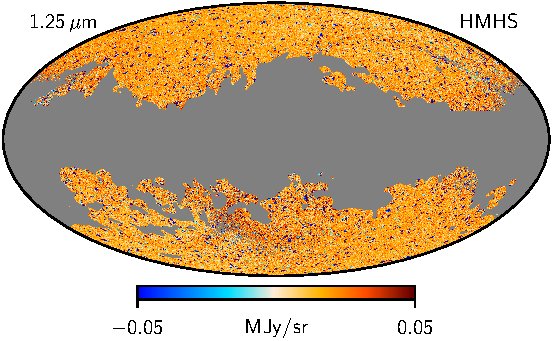
\includegraphics[width=0.42\linewidth]{figs/dirbe_01_hmhs_v1.pdf}\hspace*{5mm}
  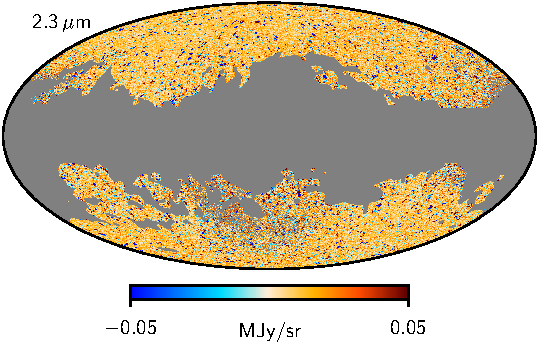
\includegraphics[width=0.42\linewidth]{figs/dirbe_02_hmhs_v1.pdf}\\
  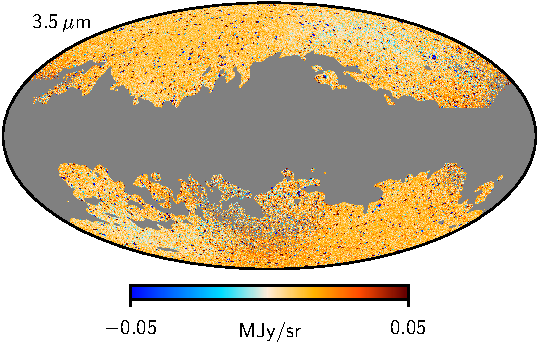
\includegraphics[width=0.42\linewidth]{figs/dirbe_03_hmhs_v1.pdf}\hspace*{5mm}
  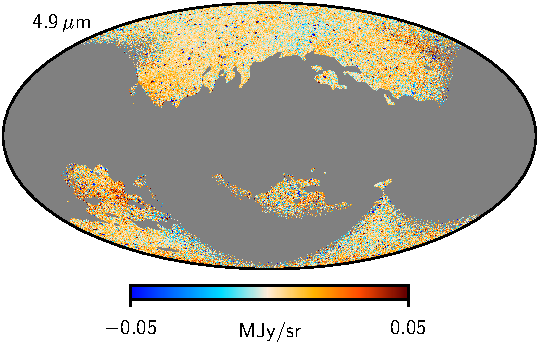
\includegraphics[width=0.42\linewidth]{figs/dirbe_04_hmhs_v1.pdf}\\
  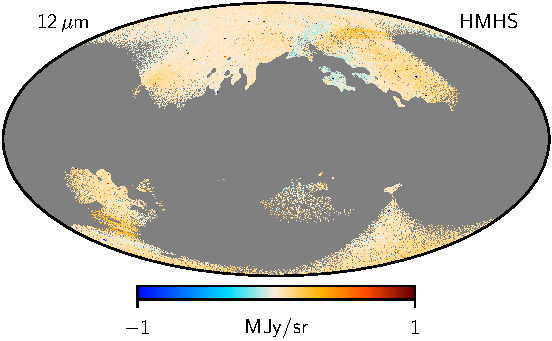
\includegraphics[width=0.42\linewidth]{figs/dirbe_05_hmhs_v1.pdf}\hspace*{5mm}
  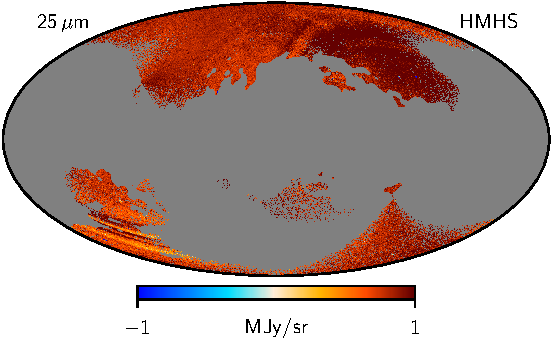
\includegraphics[width=0.42\linewidth]{figs/dirbe_06_hmhs_v1.pdf}\\
  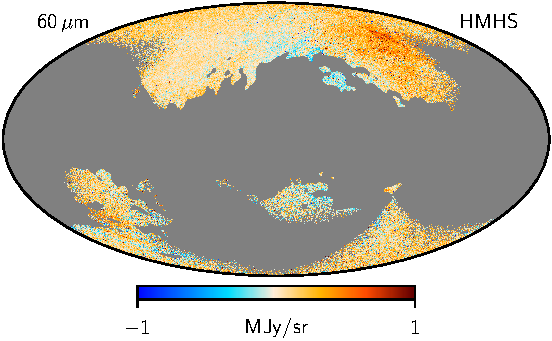
\includegraphics[width=0.42\linewidth]{figs/dirbe_07_hmhs_v1.pdf}\hspace*{5mm}
  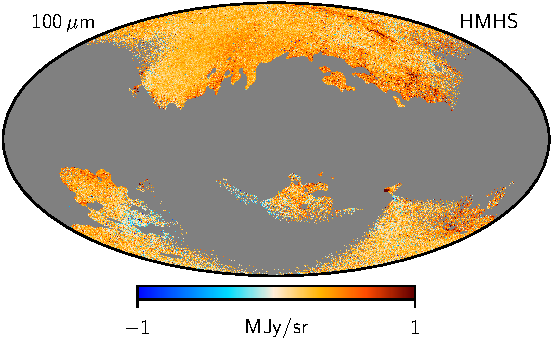
\includegraphics[width=0.42\linewidth]{figs/dirbe_08_hmhs_v1.pdf}\\
  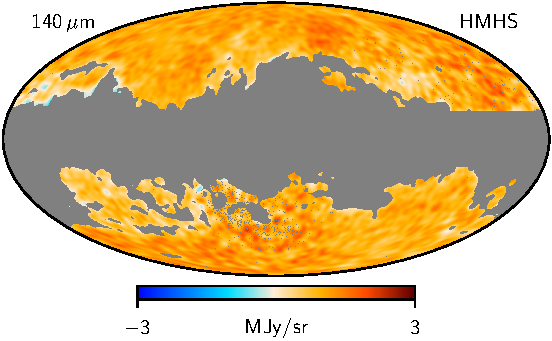
\includegraphics[width=0.42\linewidth]{figs/dirbe_09_hmhs_v1_3deg.pdf}\hspace*{5mm}
  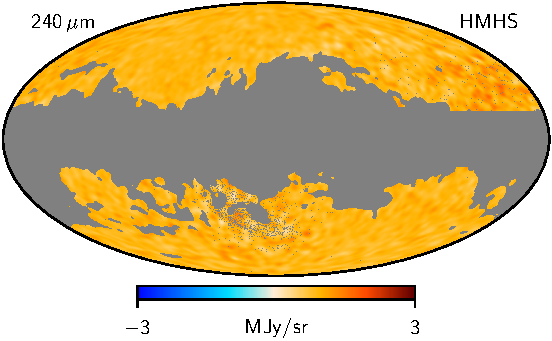
\includegraphics[width=0.42\linewidth]{figs/dirbe_10_hmhs_v1_3deg.pdf}
  \caption{Half-mission half-sum maps, $(\m_{\mathrm{HM1}}+\m_{\mathrm{HM2}})/2$ for each DIRBE frequency channel. Grey pixels indicate the union of a Galactic mask and the requirement that any pixels must be observed during both HM1 and HM2. The 140 and 240\,$\mu\mathrm{m}$ maps have been smoothed to an angular resolution of $3^{\circ}$.}
  \label{fig:hmhs}
\end{figure*}

\begin{figure*}
  \centering
  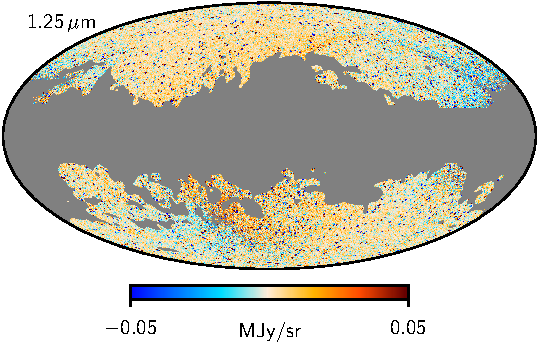
\includegraphics[width=0.42\linewidth]{figs/dirbe_01_hmhd_v1.pdf}\hspace*{5mm}
  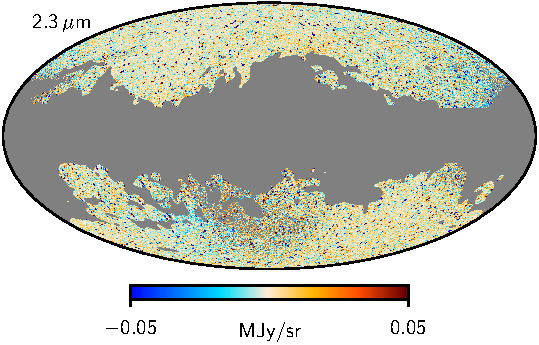
\includegraphics[width=0.42\linewidth]{figs/dirbe_02_hmhd_v1.pdf}\\
  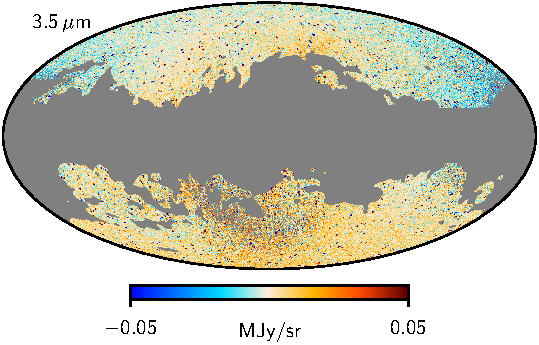
\includegraphics[width=0.42\linewidth]{figs/dirbe_03_hmhd_v1.pdf}\hspace*{5mm}
  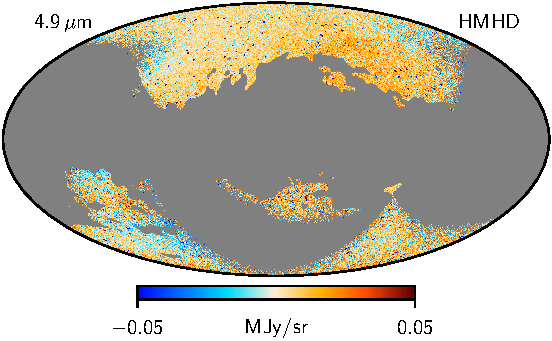
\includegraphics[width=0.42\linewidth]{figs/dirbe_04_hmhd_v1.pdf}\\
  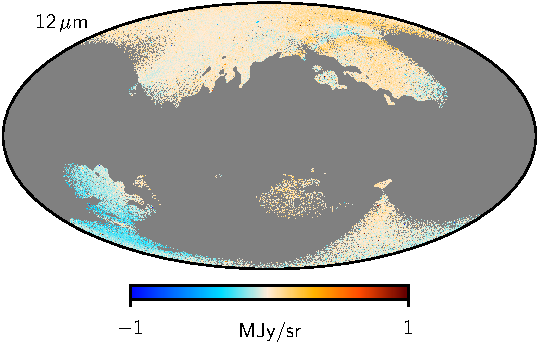
\includegraphics[width=0.42\linewidth]{figs/dirbe_05_hmhd_v1.pdf}\hspace*{5mm}
  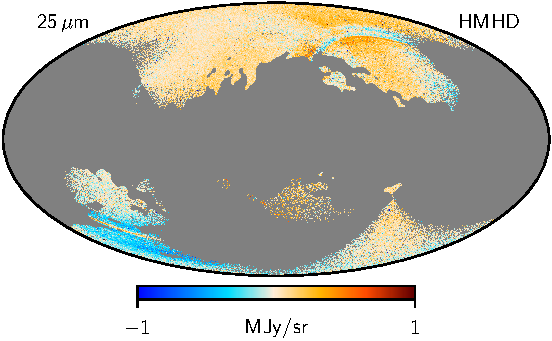
\includegraphics[width=0.42\linewidth]{figs/dirbe_06_hmhd_v1.pdf}\\
  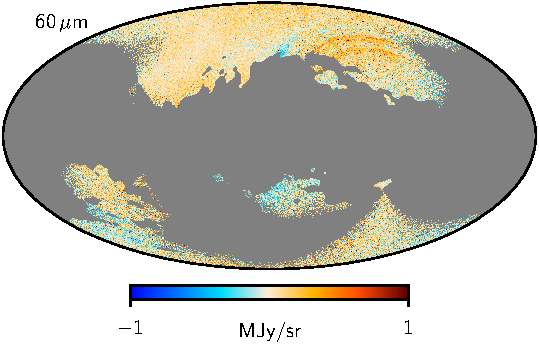
\includegraphics[width=0.42\linewidth]{figs/dirbe_07_hmhd_v1.pdf}\hspace*{5mm}
  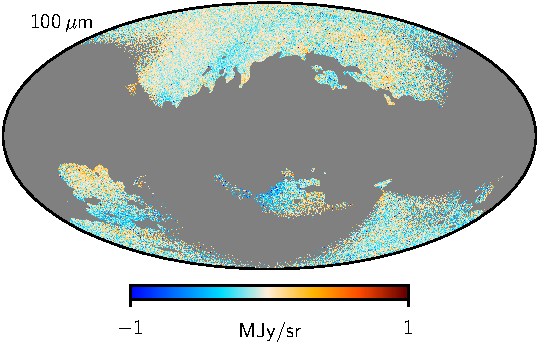
\includegraphics[width=0.42\linewidth]{figs/dirbe_08_hmhd_v1.pdf}\\
  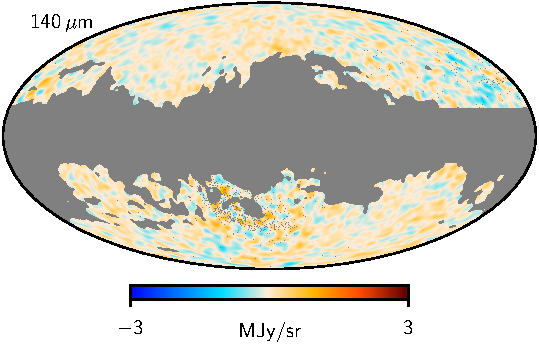
\includegraphics[width=0.42\linewidth]{figs/dirbe_09_hmhd_v1_3deg.pdf}\hspace*{5mm}
  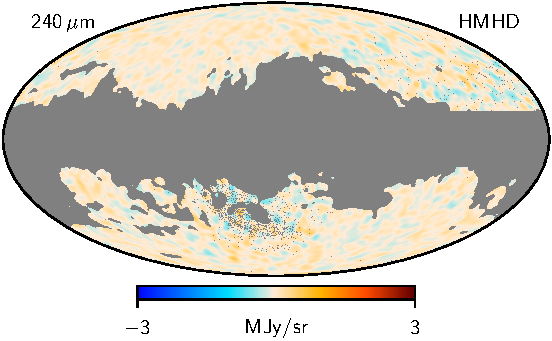
\includegraphics[width=0.42\linewidth]{figs/dirbe_10_hmhd_v1_3deg.pdf}
  \caption{Half-mission half-difference maps, $(\m_{\mathrm{HM1}}-\m_{\mathrm{HM2}})/2$ for each DIRBE frequency channel. Grey pixels indicate the union of a Galactic mask and the requirement that any pixels must be observed during both HM1 and HM2. The 140 and 240\,$\mu\mathrm{m}$ maps have been smoothed to an angular resolution of $3^{\circ}$ FWHM.}
  \label{fig:hmhd}
\end{figure*}

\subsection{Known residual systematic effects}

\begin{figure}
  \centering
  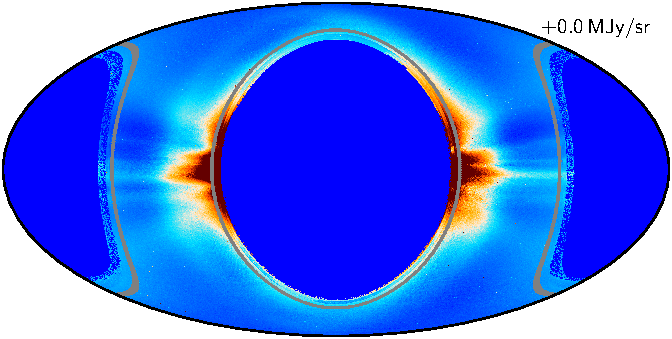
\includegraphics[width=\linewidth]{figs/solarmap_06_v1_mono0.pdf}\\
  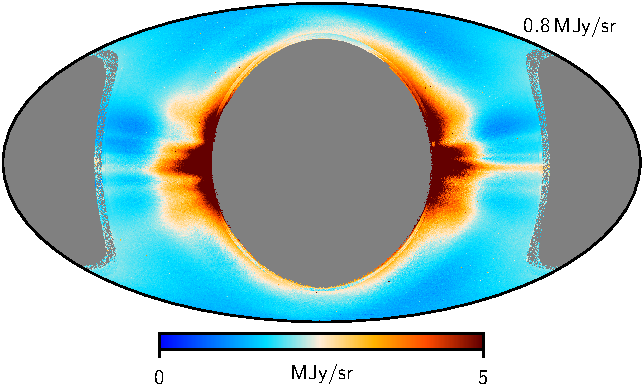
\includegraphics[width=\linewidth]{figs/solarmap_06_v1_mono8.pdf}
  \caption{(\emph{Top:}) Default solar-centric sidelobe model used in the \cosmoglobe\ DR2 analysis for the 25\,$\mu$m channel, plotted in solar-centric coordinates; see \citet{CG02_01} for full discussion. (\emph{Bottom:}) Same as above, but with an additional offset of +0.8\,MJy/sr, corresponding to the CIB monopole at 25\,$\mu$m reported in this paper.}
  \label{fig:sidelobe}
\end{figure}


\clearpage
\section{CIB monopole constraints}
\label{sec:mono}

\subsection{Algorithms}

\subsection{Markov chains and convergence}

\subsection{Results}

\subsection{Comparison with previous methods}

DIRBE was designed to detect the CIB, but the high amplitude of zodiacal light emission posed problems. As shown in \citet{CG02_02}, zodiacal light residuals in the DIRBE maps have been reduced by a factor of three in most bands using a joint analysis with a fairly restrictive model.

As shown in \citet{CG02_01}, the residuals at the $100\,\mathrm{\mu m}$ and $240\,\mathrm{\mu m}$ have well-understood noise properties, which residuals that correlate with the GNILC \citet{planck2016-XLVIII} CIB maps at 857\,GHz with $\rho=0.5\pm0.1$ at $\ell\sim200$. Much of this can be understood by using external \Planck\ HFI data to generate the sky model. 

We also use \citet{lenz2019}'s CIB maps from \Planck.

Furthermore, using the FIRAS absolutely calibrated data, we are able to ascertain the absolute zero level in both the FIRAS bands and also the DIRBE bands. At bands 60, 100, 140, and 240 $\mathrm{\mu m}$, we have confirmed the monopole to have an amplitude consistent with theoretical expectations \citep{finke2022}. At bands 12 and 25 $\mathrm{\mu m}$, zodiacal emission is brightest, so despite improving the official DIRBE ZSMA monopoles by a factor of three, the monoopoles here are clearly still dominated by zodiacal residuals. Bands 1.25, 2.2, 3.5, and 4.9 $\mathrm{\mu m}$ are closest, but here the emission is dominated by stars, many of which are fully unresolved. \citet{CG02_01} performed an analysis assuming each star is a modified blackbody, but this can certainly be improved by the physical parameters delivered by \textit{Gaia}.

\begin{figure}
  \centering
  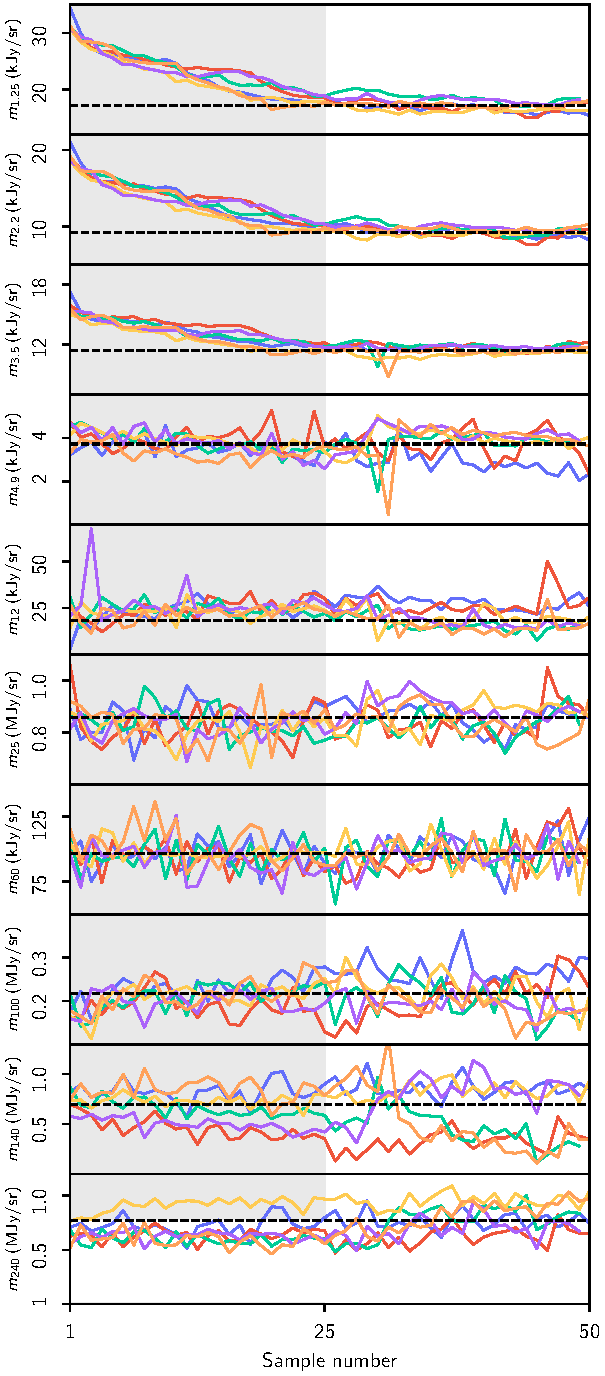
\includegraphics[width=\linewidth]{figs/traceplot_DR2_CIBmono.pdf}
  \caption{CIB monopole estimates as a function of Gibbs sample iteration for each DIRBE channel. Each color shows one Markov chain, the gray region indicates discarded burn-in, and the dashed line shows the final \Cosmoglobe\ DR2 posterior mean values as tabulated in Table~\ref{tab:CIB_monopole}.  }
  \label{fig:traceplot}
\end{figure}



%\section{Maps and Residuals}
%\label{sec:maps_and_residuals}

%\lipsum 



\begin{figure*}
  \centering
  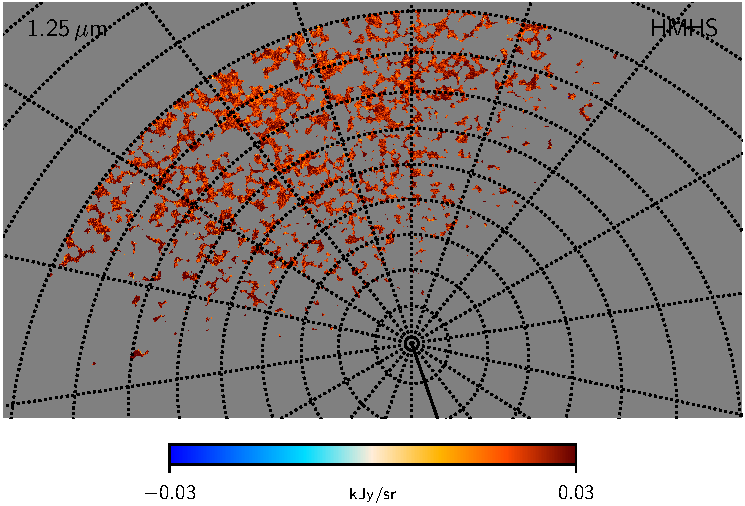
\includegraphics[width=0.38\linewidth]{figs/CGDR2_01_hmhs_fullres.pdf}\hspace*{5mm}
  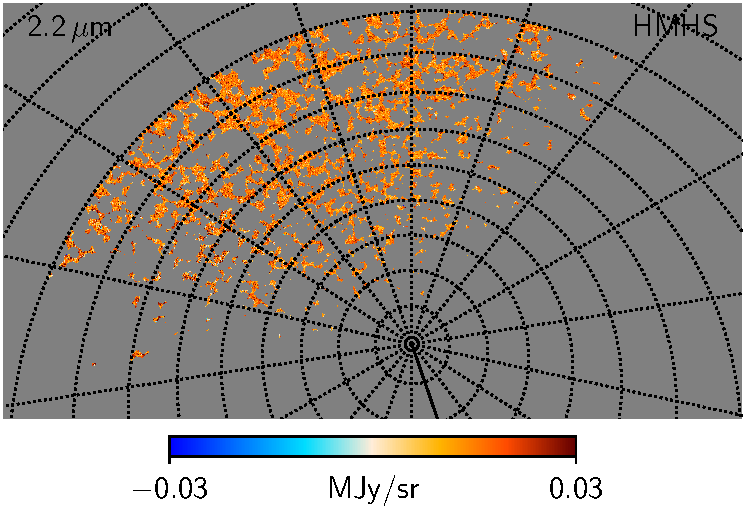
\includegraphics[width=0.38\linewidth]{figs/CGDR2_02_hmhs_fullres.pdf}\\
  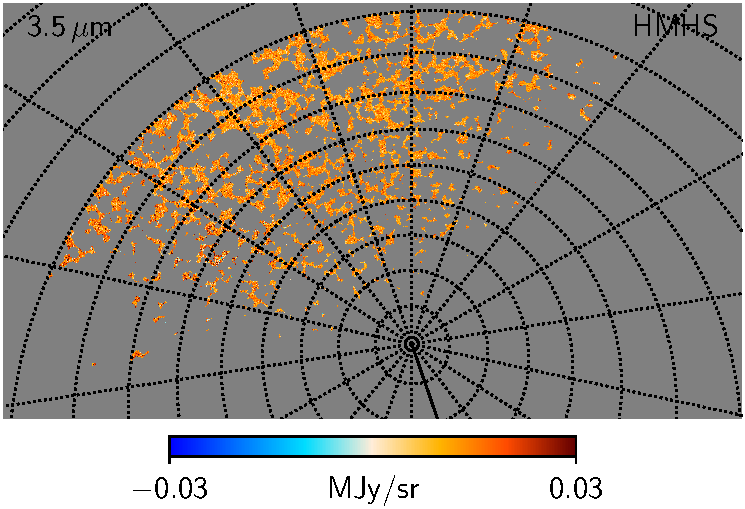
\includegraphics[width=0.38\linewidth]{figs/CGDR2_03_hmhs_fullres.pdf}\hspace*{5mm}
  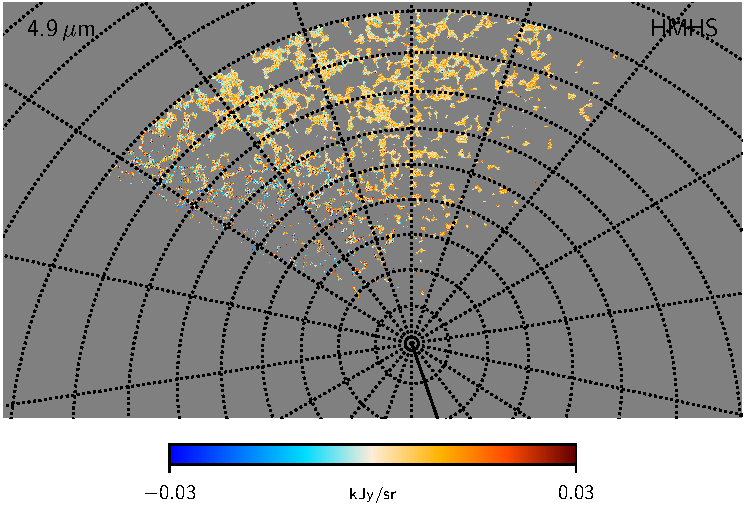
\includegraphics[width=0.38\linewidth]{figs/CGDR2_04_hmhs_fullres.pdf}\\
  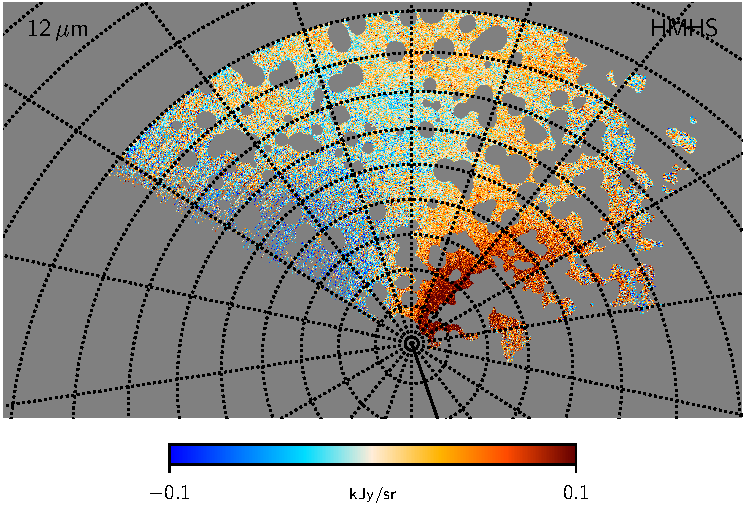
\includegraphics[width=0.38\linewidth]{figs/CGDR2_05_hmhs_fullres.pdf}\hspace*{5mm}
  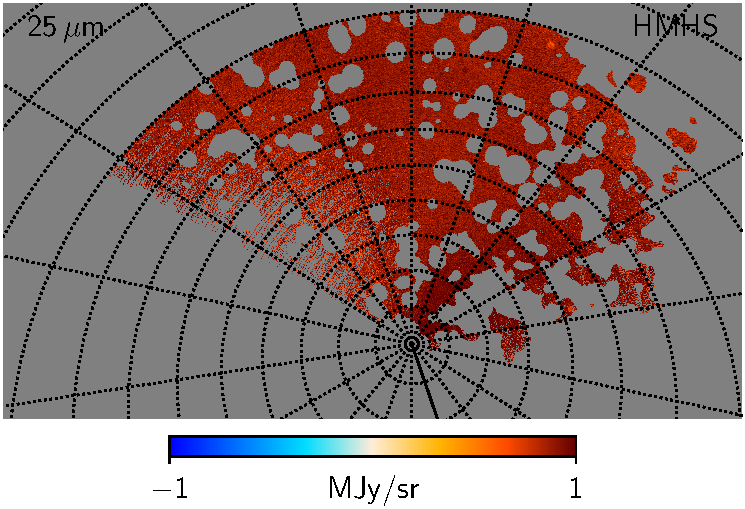
\includegraphics[width=0.38\linewidth]{figs/CGDR2_06_hmhs_fullres.pdf}\\
  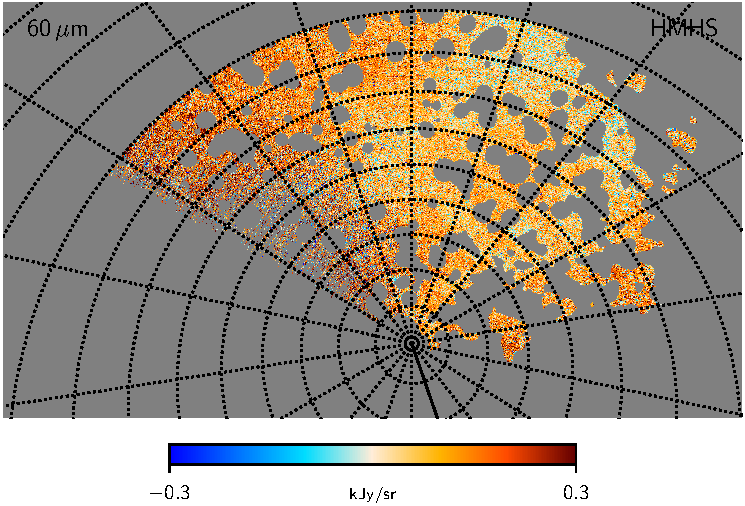
\includegraphics[width=0.38\linewidth]{figs/CGDR2_07_hmhs_fullres.pdf}\hspace*{5mm}
  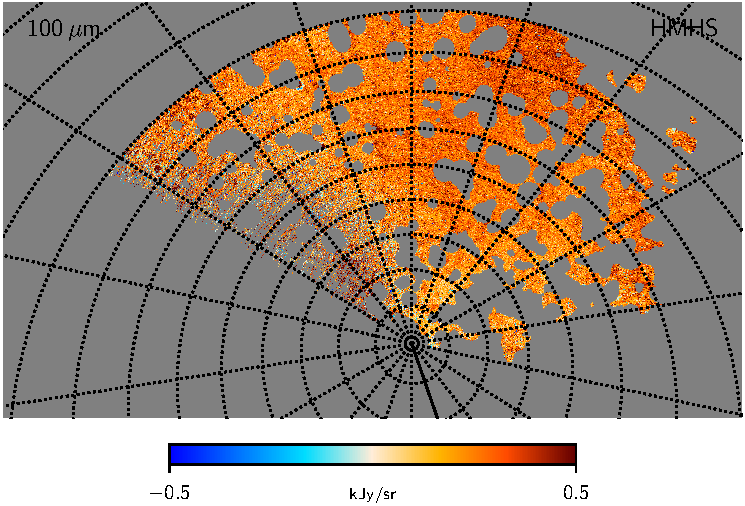
\includegraphics[width=0.38\linewidth]{figs/CGDR2_08_hmhs_fullres.pdf}\\
  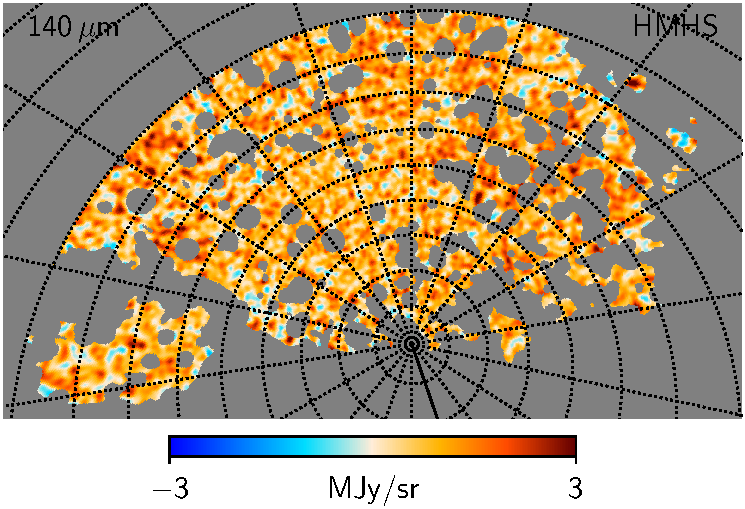
\includegraphics[width=0.38\linewidth]{figs/CGDR2_09_hmhs_fullres_1deg.pdf}\hspace*{5mm}
  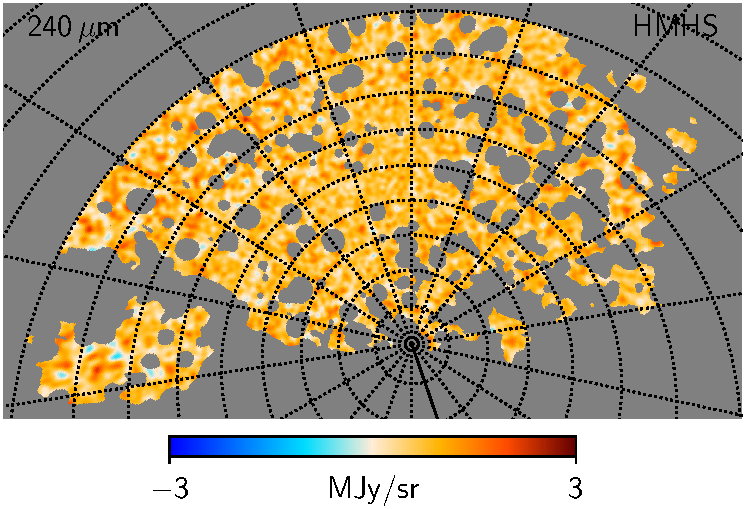
\includegraphics[width=0.38\linewidth]{figs/CGDR2_10_hmhs_fullres_1deg.pdf}
  \caption{Half-mission half-sum maps, $(\m_{\mathrm{HM1}}+\m_{\mathrm{HM2}})/2$ for each DIRBE frequency channel, zoomed in around the North Ecliptic Pole. Grey pixels indicate the conservative masks used for estimating the monopole. The graticule is centered on the NEP, and the spacing is $5^{\circ}$. The 140 and 240\,$\mu\mathrm{m}$ maps have been smoothed to an angular resolution of $1^{\circ}$ FWHM.} 
  \label{fig:hmhs_zoom}
\end{figure*}

\begin{figure*}
  \centering
  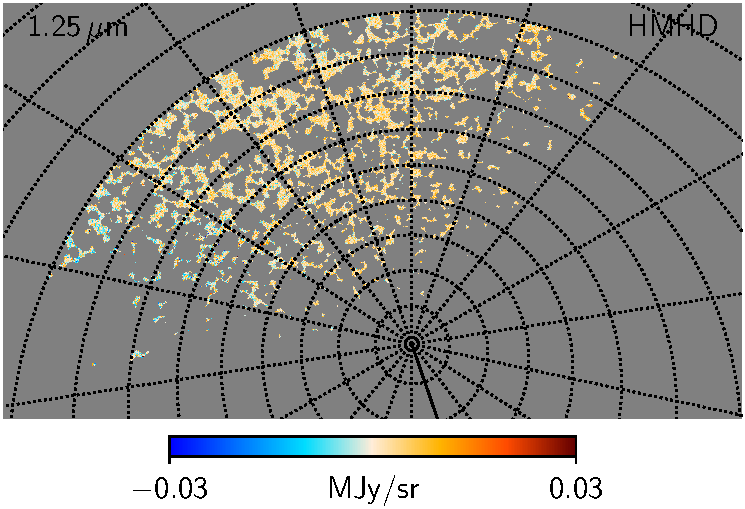
\includegraphics[width=0.38\linewidth]{figs/CGDR2_01_hmhd_fullres.pdf}\hspace*{5mm}
  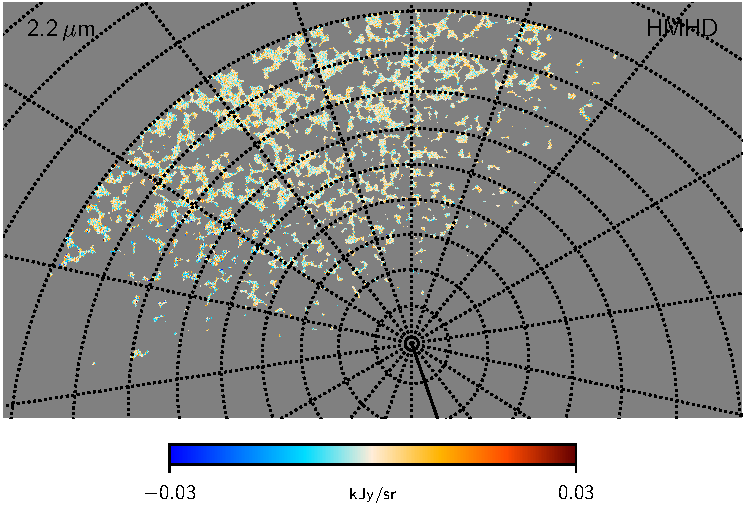
\includegraphics[width=0.38\linewidth]{figs/CGDR2_02_hmhd_fullres.pdf}\\
  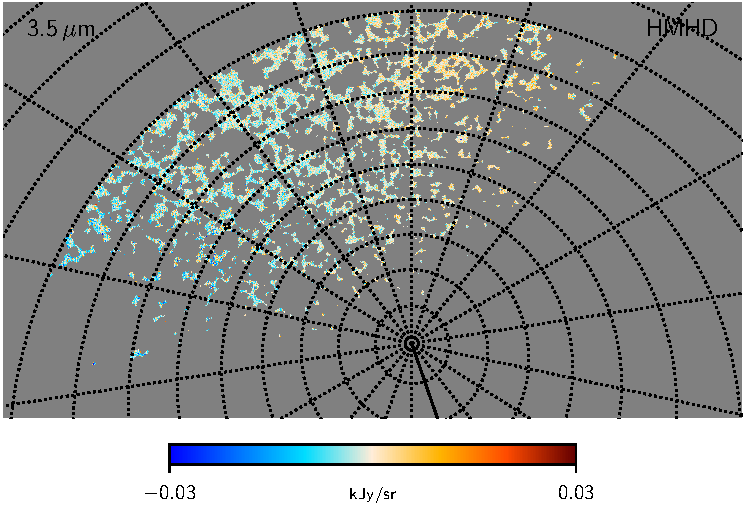
\includegraphics[width=0.38\linewidth]{figs/CGDR2_03_hmhd_fullres.pdf}\hspace*{5mm}
  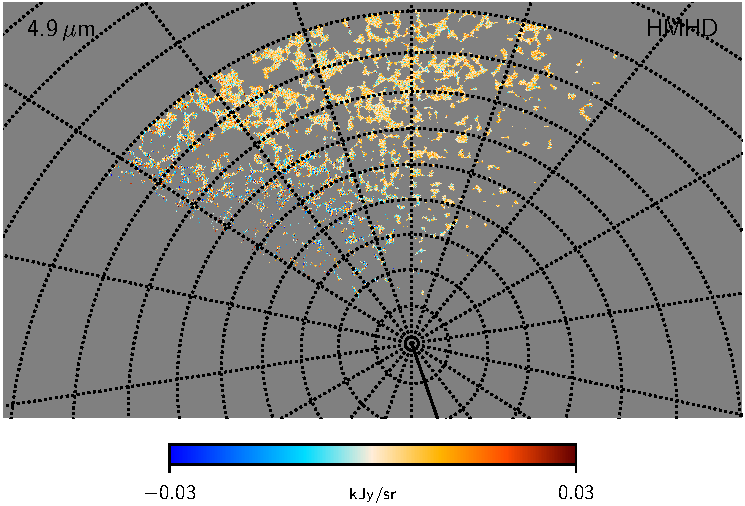
\includegraphics[width=0.38\linewidth]{figs/CGDR2_04_hmhd_fullres.pdf}\\
  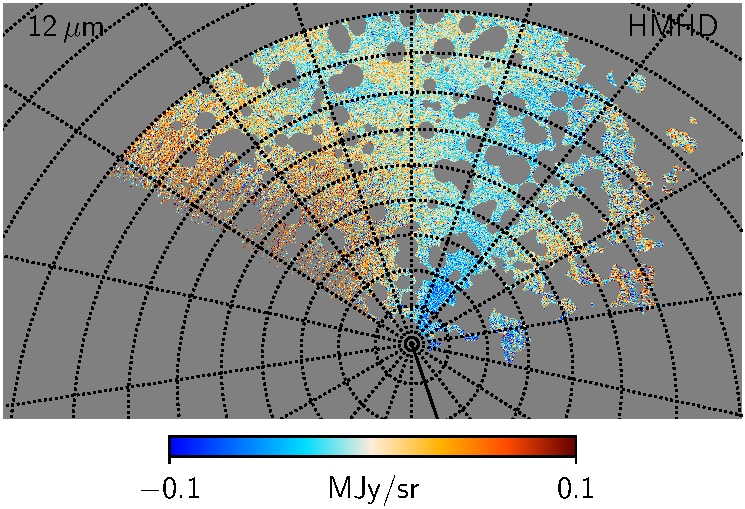
\includegraphics[width=0.38\linewidth]{figs/CGDR2_05_hmhd_fullres.pdf}\hspace*{5mm}
  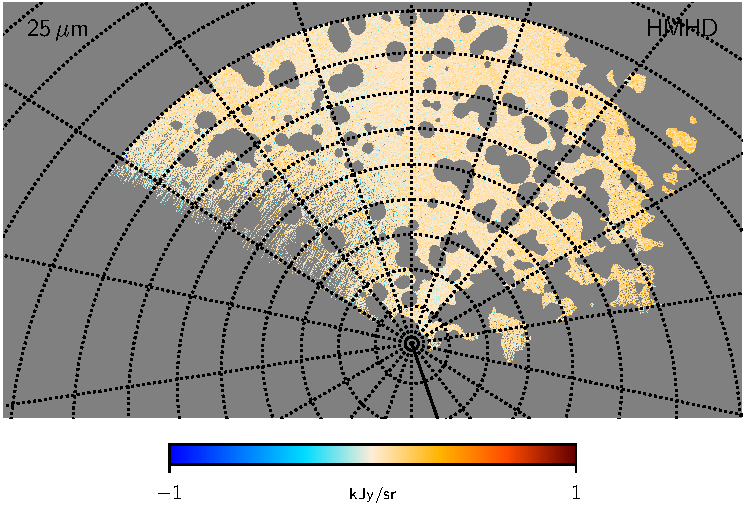
\includegraphics[width=0.38\linewidth]{figs/CGDR2_06_hmhd_fullres.pdf}\\
  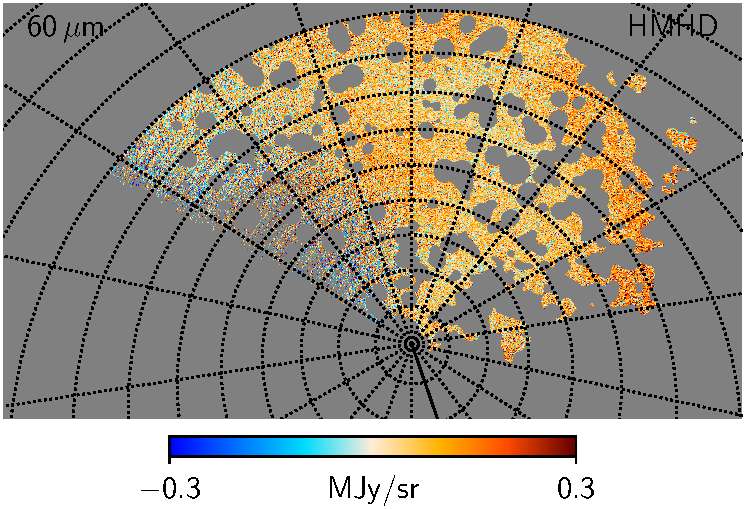
\includegraphics[width=0.38\linewidth]{figs/CGDR2_07_hmhd_fullres.pdf}\hspace*{5mm}
  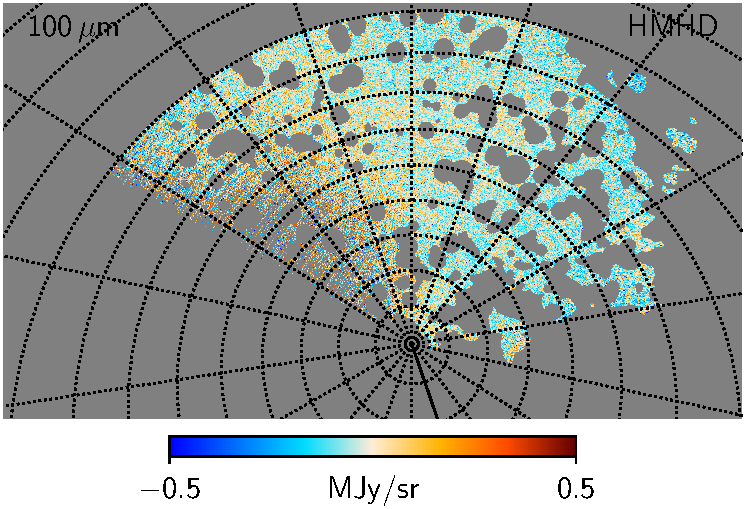
\includegraphics[width=0.38\linewidth]{figs/CGDR2_08_hmhd_fullres.pdf}\\
  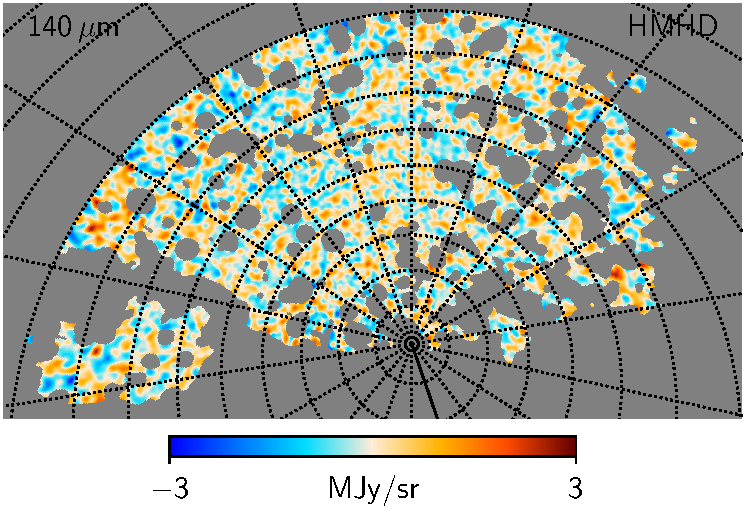
\includegraphics[width=0.38\linewidth]{figs/CGDR2_09_hmhd_fullres_1deg.pdf}\hspace*{5mm}
  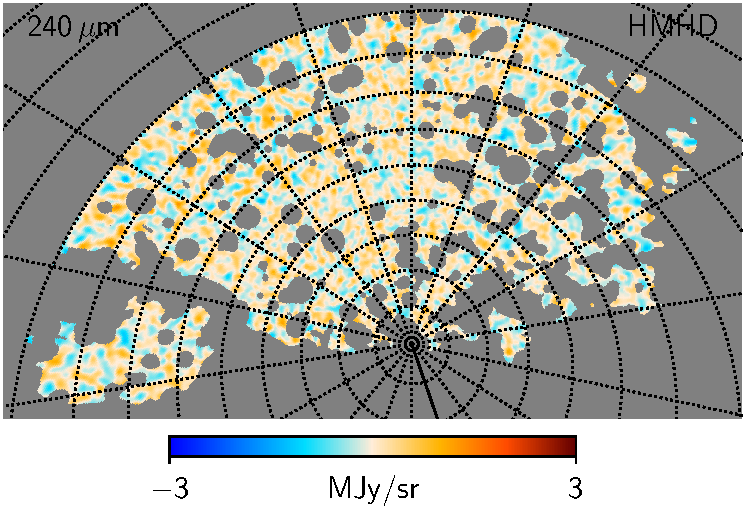
\includegraphics[width=0.38\linewidth]{figs/CGDR2_10_hmhd_fullres_1deg.pdf}
  \caption{Half-mission half-difference maps, $(\m_{\mathrm{HM1}}-\m_{\mathrm{HM2}})/2$ for each DIRBE frequency channel, zoomed in around the North Ecliptic Pole. Grey pixels indicate the conservative masks used for estimating the monopole. The graticule is centered on the NEP, and the grid spacing is $5^{\circ}$. The 140 and 240\,$\mu\mathrm{m}$ maps have been smoothed to an angular resolution of $1^{\circ}$ FWHM.}
  \label{fig:hmhd_zoom}
\end{figure*}

\begin{table*}
\newdimen\tblskip \tblskip=5pt
\caption{Summary of CIB monopole constraints and uncertainties. All numbers are given in units of $\nWmsr$. For channels with a robust monopole detection, the central value corresponds to the posterior mean of all accepted Gibbs samples, and the uncertainty is given in column (7); for channels without a robust monopole detection, the upper limit is defined as the sum of the posterior mean value and twice the uncertainty.uncertainty.  }
\label{tab:CIB_monopole}
\vskip -4mm
\footnotesize
\setbox\tablebox=\vbox{
 \newdimen\digitwidth
 \setbox0=\hbox{\rm 0}
 \digitwidth=\wd0
 \catcode`*=\active
 \def*{\kern\digitwidth}
%
  \newdimen\dpwidth
  \setbox0=\hbox{.}
  \dpwidth=\wd0
  \catcode`!=\active
  \def!{\kern\dpwidth}
%
  \halign{\hbox to 2.0cm{#\leaderfil}\tabskip 2em&
    \hfil$#$\hfil \tabskip 1em& % Uncertainty
    \hfil$#$\hfil \tabskip 1em&
    \hfil$#$\hfil \tabskip 1em& 
    \hfil$#$\hfil \tabskip 1em&
    \hfil$#$\hfil \tabskip 1em&
    \hfil$#$\hfil \tabskip 2em&
    \hfil$#$\hfil \tabskip 2em&
    \hfil$#$\hfil \tabskip 1em& % CIB constraints
    \hfil$#$\hfil \tabskip 0em\cr
\noalign{\doubleline}
\omit&\multispan6\hfil\sc Monopole uncertainty\hfil&\multispan2\hfil\sc CIB monopole constraint\hfil\cr
\noalign{\vskip -3pt}
\omit&\multispan6\hrulefill&\multispan3\hrulefill\cr
\noalign{\vskip 3pt} 
\omit\sc Wavelength ($\mu\mathrm{m}$)\hfil& \sigma_b^{\mathrm{(a)}} & \sigma_g^{\mathrm{(b)}} & \sigma_\mathrm{MC}^{\mathrm{(c)}} & \sigma_\mathrm{HM}^{\mathrm{(d)}}  & \sigma_\mathrm{SL}^{\mathrm{(e)}}  & \sigma_\mathrm{Total}^{\mathrm{(f)}}  & \mathrm{DIRBE}^{\mathrm{(g)}} & \mathrm{Gibbs}^{(h)} & \mathrm{CG\, DR2}^{(i)} \cr
\noalign{\vskip 3pt\hrule\vskip 5pt}
*1.25 & 0.05 & 1.3 & 2.0 &  5.9   & *0 & *6!* & <75        & *57\pm0 & *41\pm6 \cr
*2.2  & 0.03 & 0.4 & 0.7 &  1.3   & *0 & *1.5 & <39        & *20\pm0 & *13\pm2 \cr
*3.5  & 0.02 & 0.3 & 0.2 &  1.5   & *0 & *1.5 & <23        & **9\pm0 & *10\pm2 \cr
*4.9  & 0.01 & 0.1 & 0.3 &  2.0   & *3 & *3!* & <41        & **<3 & **<8 \cr
*12   & 0.02 & 0.3 & 0.9 &  0.4   & 19 & 19!* & <468       & **>7 & *<45 \cr
*25   & 0.01 & 15 & 4.0 &  4.9    & 11 & 20!* & <504       & >100 & <140 \cr
*60   & 1.34 & 0.5 & 0.5 &  3.0   & *1 & *4!* & <75        & **>4 & *<13 \cr
100   & 0.81 & 1.0 & 1.0 &  1.3   & 11 & 11!* & <34        & **>7 & *<29 \cr
140   & 5!**  & 1.4 & 4.0 &  0.1  & *0 & *7!* & 25.0\pm6.9 & *14\pm0 & *13\pm7 \cr
240   & 2!**  & 1.0 & 1.1 &  0.8  & *0 & *3!* & 13.6\pm2.5 & **9\pm0 & **9\pm3 \cr
\noalign{\vskip 5pt\hrule\vskip 5pt}}}
\endPlancktablewide
\tablenote {{\rm a}} CIO baseline (or offset) uncertainty as estimated by the DIRBE team; reproduced from Table~1 of \citet{hauser:1998}.\par
\tablenote {{\rm b}} CIO gain uncertainty; estimated by multiplying the gain uncertainty in Table~1 of \citet{hauser:1998} with the \cosmoglobe\ posterior mean values listed in the ninth column.\par
\tablenote {{\rm c}} Statistical Monte Carlo uncertainty estimated as the standard deviation of all accepted Gibbs samples; accounts for astrophysical and zodiacal light uncertainties.\par
\tablenote {{\rm d}} Systematic monopole uncertainty, defined as the mean absolute difference between individual HM1 and HM2 estimates; accounts for zodiacal light modelling errors and potential instrumental drifts.\par
\tablenote {{\rm e}} Systematic monopole uncertainty from the unknown zero-level of the sidelobe model.\par
\tablenote {{\rm f}} Total monopole uncertainty obtained by adding columns (2)--(6) in quadrature.\par
\tablenote {{\rm g}} Official DIRBE monopole constraints reproduced from Table~1 of \citet{hauser:1998}.\par
\tablenote {{\rm h}} \cosmoglobe\ DR2 CIB constraint as derived directly from the monopole parameter in the Gibbs chain; see \citet{CG02_01}.\par
\tablenote {{\rm i}} \cosmoglobe\ DR2 CIB constraint as derived with the tuned CIB monopole estimator discussed in Sect.~\ref{sec:mono}. This uses a more conservative mask than the Gibbs chain result in column (9), and we consider this as the final result.\par
\par
\end{table*}


\begin{figure*}
	\centering
	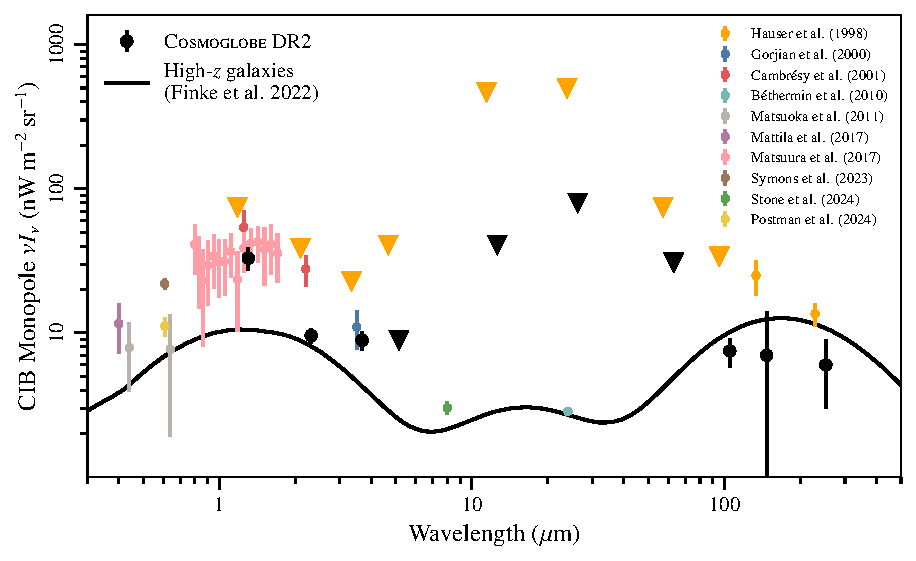
\includegraphics[width=0.8\textwidth]{figs/CIB_mono.pdf}
	\caption{Monopoles as measured by DIRBE, compared with theoretical predictions for EBL. Empty circles are DIRBE ZSMA maps with \textsc{Cosmoglobe} sky model removed.}
	\label{fig: EBL_monopoles}
\end{figure*}



%\begin{figure*}
%  \centering
%  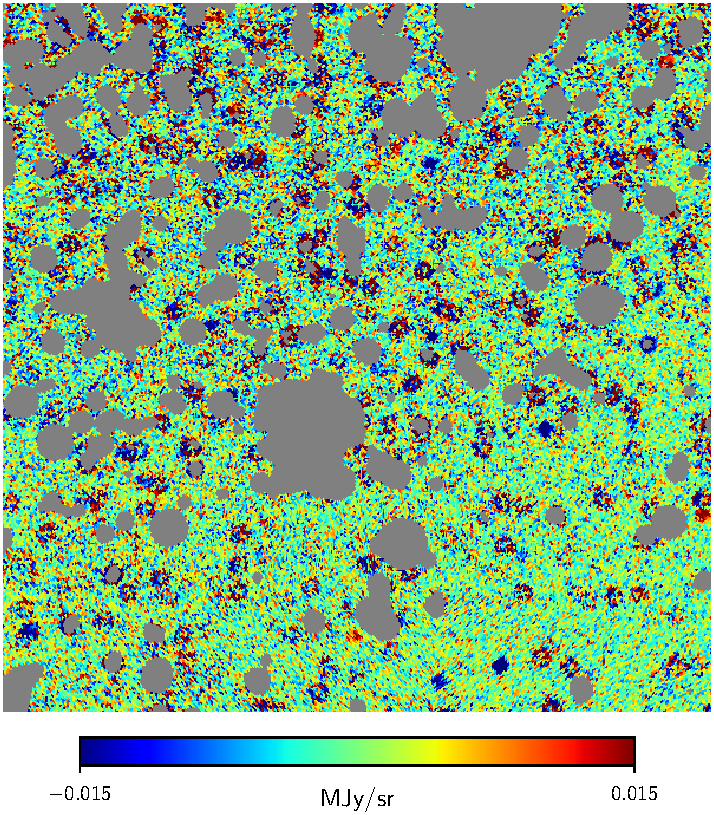
\includegraphics[width=0.23\linewidth]{figs/dirbe_01_hmhd_v1_zoom.pdf}\hspace*{5mm}
%  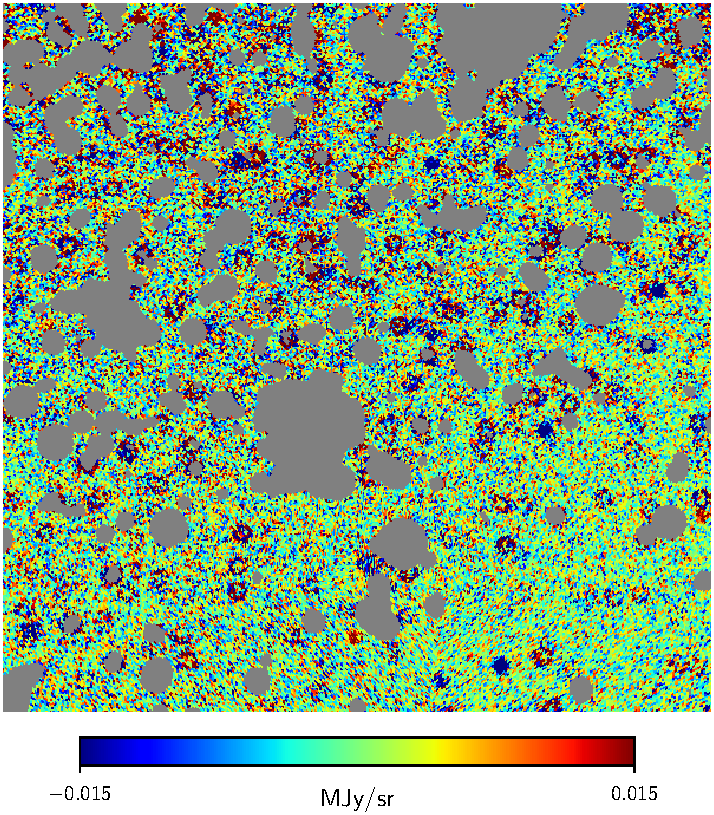
\includegraphics[width=0.23\linewidth]{figs/dirbe_02_hmhd_v1_zoom.pdf}\\
%  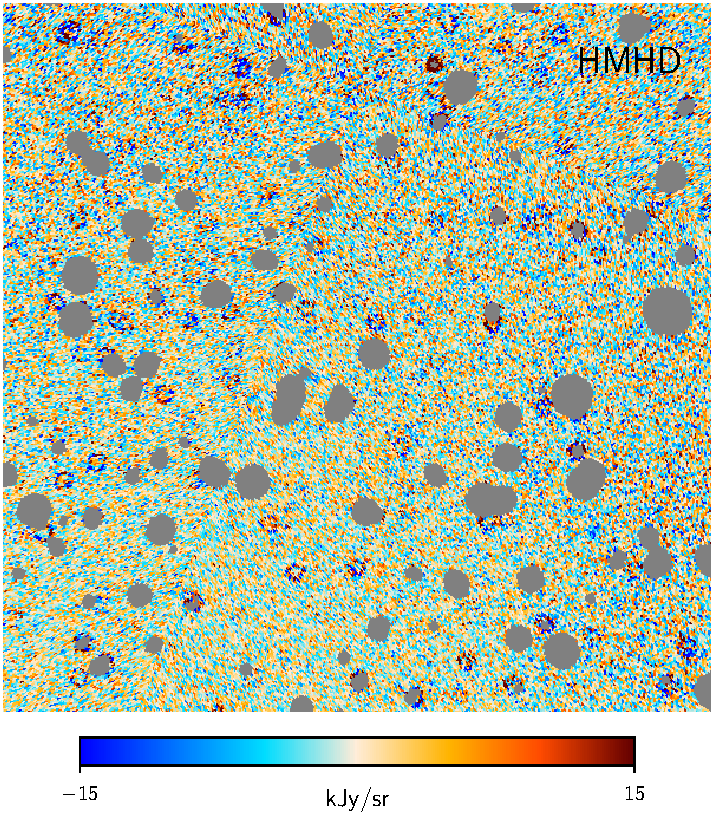
\includegraphics[width=0.23\linewidth]{figs/dirbe_03_hmhd_v1_zoom.pdf}\hspace*{5mm}
%  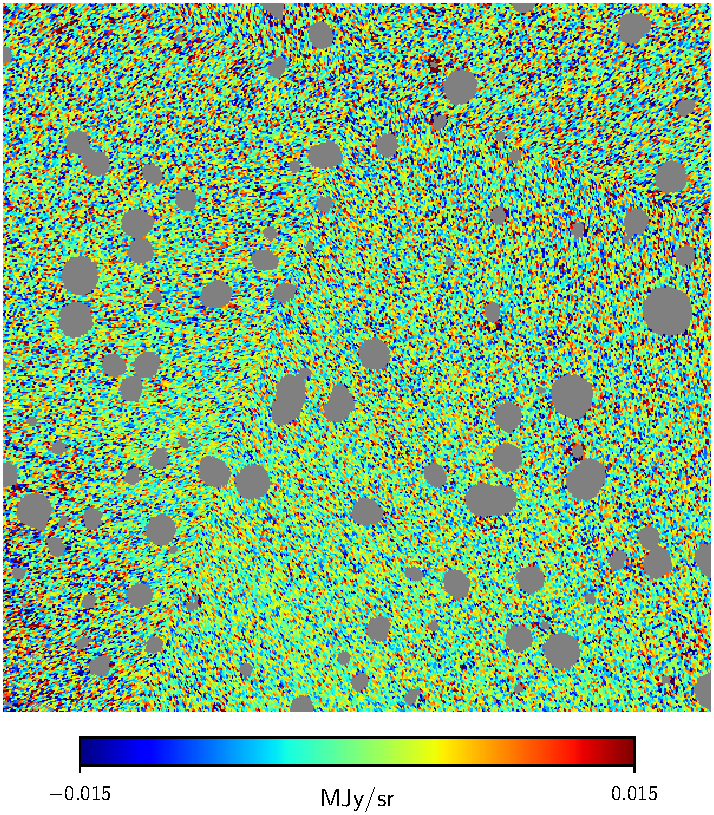
\includegraphics[width=0.23\linewidth]{figs/dirbe_04_hmhd_v1_zoom.pdf}\\
%  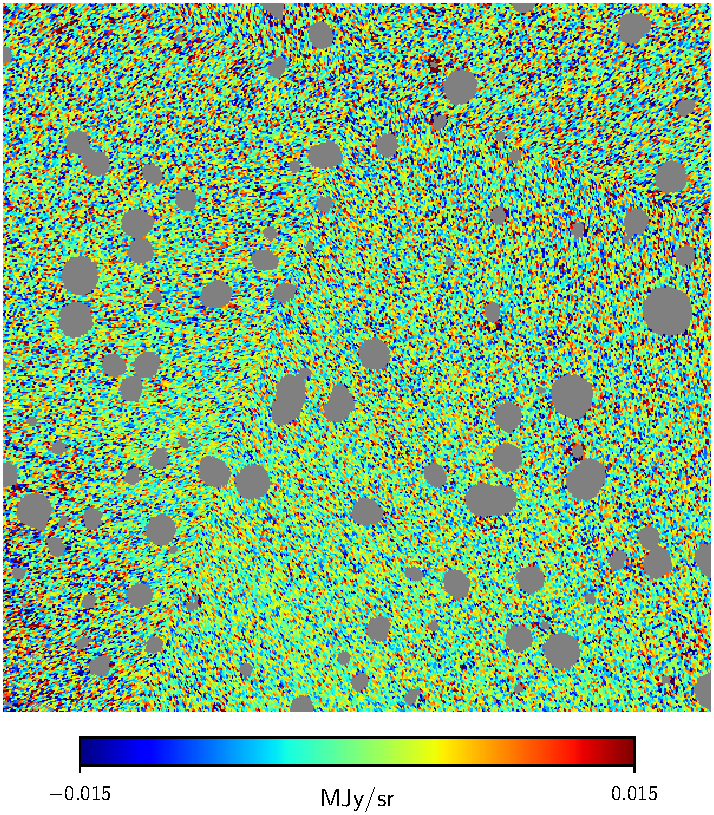
\includegraphics[width=0.23\linewidth]{figs/dirbe_04_hmhd_v1_zoom.pdf}\hspace*{5mm}
%  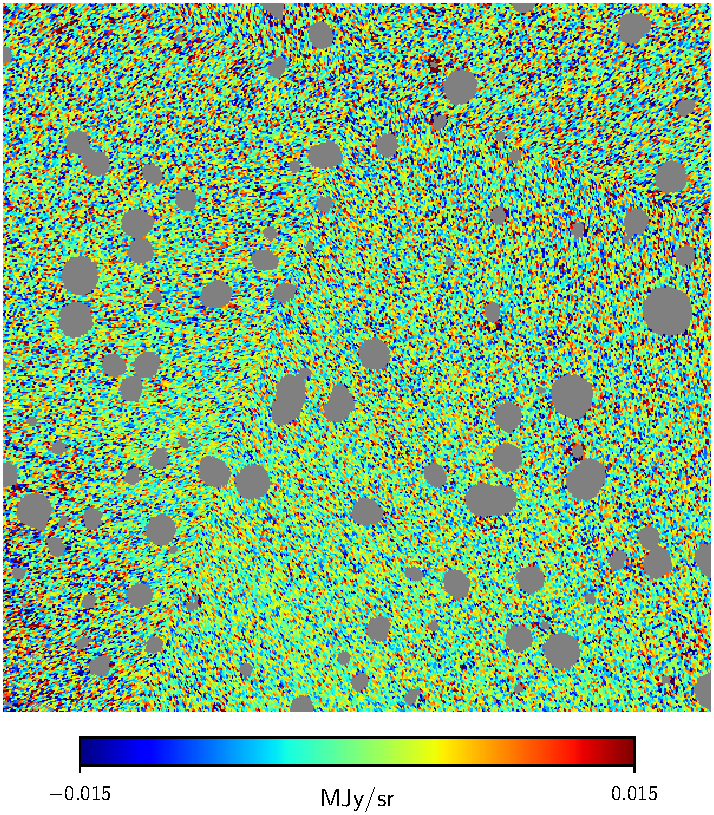
\includegraphics[width=0.23\linewidth]{figs/dirbe_04_hmhd_v1_zoom.pdf}\\
%  \includegraphics[width=0.23\linewidth]{figs/dirbe_04_hmhd_v1_zoom.pdf}\hspace*{5mm}
%  \includegraphics[width=0.23\linewidth]{figs/dirbe_04_hmhd_v1_zoom.pdf}\\
%  \includegraphics[width=0.23\linewidth]{figs/dirbe_04_hmhd_v1_zoom.pdf}\hspace*{5mm}
%  \includegraphics[width=0.23\linewidth]{figs/dirbe_04_hmhd_v1_zoom.pdf}
%  \caption{Zoom-ins centered on Galactic coordinates $(l,b)=(90^{\circ},80^{\circ})$ of the half-mission half-sum maps, $(\m_{\mathrm{HM1}}+\m_{\mathrm{HM2}})/2$ for each DIRBE frequency channel. }
%  \label{fig:hmhd_zoom}
%\end{figure*}

%\begin{figure}
%	\centering
%	\includegraphics[width=\columnwidth]{figs/patch_04.pdf}
%	\includegraphics[width=\columnwidth]{figs/patch_07.pdf}
%	\includegraphics[width=\columnwidth]{figs/patch_08.pdf}
%	\caption{Half-sum and half-difference maps centered at $(l,b)=(67^\circ,56^\circ)$.}
%\end{figure}

%\section{Monopoles}
%\label{sec:mono}







%Monopole values, comparison with zodi values, compared with theoretical predictions, previous limits, and previous detections.

\clearpage
\section{CIB anisotropies}
\label{sec:fluct}

Power spectra, comparison with GNILC, compare with theoretical predictions, previous limits, and previous detections.

\subsection{Map-domain fluctuations}

\begin{figure*}
  \centering
  %\includegraphics[width=0.23\linewidth]{figs/dirbe_01_hmhs_v1_zoom.pdf}\hspace*{5mm}
  %\includegraphics[width=0.23\linewidth]{figs/dirbe_02_hmhs_v1_zoom.pdf}\\
  \includegraphics[width=0.45\linewidth]{figs/CGDR2_03_hmhs_filter_15arc_5deg.pdf}\hspace*{0mm}
  \includegraphics[width=0.45\linewidth]{figs/CGDR2_03_hmhd_filter_15arc_5deg.pdf}
  %\includegraphics[width=0.45\linewidth]{figs/dirbe_03_hmhd_v1_zoom.pdf}\hspace*{5mm}
  %\includegraphics[width=0.45\linewidth]{figs/dirbe_04_hmhd_v1_zoom.pdf}
  %\includegraphics[width=0.23\linewidth]{figs/dirbe_04_hmhs_v1_zoom.pdf}\hspace*{5mm}
  %\includegraphics[width=0.23\linewidth]{figs/dirbe_04_hmhs_v1_zoom.pdf}\\
  %\includegraphics[width=0.23\linewidth]{figs/dirbe_04_hmhs_v1_zoom.pdf}\hspace*{5mm}
  %\includegraphics[width=0.23\linewidth]{figs/dirbe_04_hmhs_v1_zoom.pdf}\\
  %\includegraphics[width=0.23\linewidth]{figs/dirbe_04_hmhs_v1_zoom.pdf}\hspace*{5mm}
  %\includegraphics[width=0.23\linewidth]{figs/dirbe_04_hmhs_v1_zoom.pdf}
  \caption{Zoom-ins centered of the inverse noise weighted full-mission (\emph{left}) and half-mission half-difference (\emph{right}) residual maps at $3.5\,\mu\mathrm{m}$. Both maps are bandpass filtered to remove scales larger than $5^{\circ}$ FWHM and smaller than $15'$ FWHM, and plotted in Galactic coordinates centered on $(l,b)=(70^{\circ},75^{\circ})$. The graticule corresponds to Ecliptic coordinates, and the grid spacing is $5^{\circ}$. The rms of the left and right maps are 2.6 and 2.2\,$\mathrm{kJy}/\mathrm{sr}$, respectively. }
  \label{fig:hmhs_zoom_fluct}
\end{figure*}

\subsection{Power spectrum constraints}


\section{Conclusions}
\label{sec:conclusions}

This is the first time that CIB fluctuations have been detected in DIRBE, and the first time that fluctuations and monopoles have been detected in the same band.

As demonstrated here, the limitation in fully modeling the CIB has been the inability to properly utilize external data. In this work, the reanalysis of DIRBE data was made much simpler not only by the large increase of relative computing power with respect to dataset size, but also the information gained by using a global sky model spanning from $100\,\mathrm{GHz}$ to $1\,\mathrm{\mu m}$.

Much of this work is made possible through the use of archival time-ordered data with complementary scan strategies, frequency coverage, detector technologies, and observation time. In the case of CIB studies, the interplay between foregrounds, namely zodiacal and Galactic dust, has limited previous detections. In future work, additional data will further break these degeneracies, and the potential to further understand the astrophysical signals in these datasets will be improved. In particular, the \textit{Infrared Astrophysical Observatory} (\textit{IRAS}) created nearly full-sky maps at 12, 25, 60, and 100 $\mathrm{\mu m}$ with resolution between 0.5 arcmin to 2 arcmin. A full end-to-end joint analysis of \textit{IRAS} and DIRBE will leverage the unique properties of both datsets, and enable an even deeper view of the CIB in the tens of microns.

\begin{acknowledgements}
 The current work has received funding from the European
  Union’s Horizon 2020 research and innovation programme under grant
  agreement numbers 819478 (ERC; \textsc{Cosmoglobe}) and 772253 (ERC;
	\textsc{bits2cosmology}). Some of the results in this paper have been derived using healpy \citep{Zonca2019} and the HEALPix \citep{healpix} package.
  We acknowledge the use of the Legacy Archive for Microwave Background Data
  Analysis (LAMBDA), part of the High Energy Astrophysics Science Archive Center
  (HEASARC). HEASARC/LAMBDA is a service of the Astrophysics Science Division at
  the NASA Goddard Space Flight Center.  
\end{acknowledgements}


%-------------------------------------------------------------
%                                       Table with references 
%-------------------------------------------------------------
%

\bibliographystyle{aa}
\bibliography{../../common/Planck_bib,../../common/CG_bibliography}

\end{document}
%%%% End of aa.dem

\begin{table*}
\newdimen\tblskip \tblskip=5pt
\caption{Summary of CIB monopole constraints and uncertainties. All numbers are given in units of \nWmsr, except the gain uncertainty $\sigma_{\mathrm{g}}$, which is given in units of percent. }
\label{tab:CIB_monopole_v2}
\vskip -4mm
\footnotesize
\setbox\tablebox=\vbox{
 \newdimen\digitwidth
 \setbox0=\hbox{\rm 0}
 \digitwidth=\wd0
 \catcode`*=\active
 \def*{\kern\digitwidth}
%
  \newdimen\dpwidth
  \setbox0=\hbox{.}
  \dpwidth=\wd0
  \catcode`!=\active
  \def!{\kern\dpwidth}
%
  \halign{\hbox to 2.0cm{#\leaderfil}\tabskip 2em&
    \hfil$#$\hfil \tabskip 1em& % Instrument
    \hfil$#$\hfil \tabskip 2em&
    \hfil$#$\hfil \tabskip 1em& % Uncertainty
    \hfil$#$\hfil \tabskip 1em&
    \hfil$#$\hfil \tabskip 1em&
    \hfil$#$\hfil \tabskip 1em&
    \hfil$#$\hfil \tabskip 1em& % CIB constraints
    \hfil$#$\hfil \tabskip 0em\cr
\noalign{\doubleline}
\omit&\multispan2\hfil\sc Instrument\hfil&\multispan4\hfil\sc Monopole uncertainty\hfil&\multispan2\hfil\sc CIB monopole constraint\hfil\cr
\noalign{\vskip -3pt}
\omit&\multispan2\hrulefill&\multispan4\hrulefill&\multispan2\hrulefill\cr
\noalign{\vskip 3pt} 
\omit\sc Wavelength ($\mu\mathrm{m}$)\hfil& \sigma_{\mathrm{wn}} & \sigma_{g}^{(\mathrm{a})} (\%) & \mathrm{MC}^{\mathrm{(b)}} & \mathrm{HM}^{\mathrm{(c)}}  & \mathrm{SL}^{\mathrm{(d)}}  & \mathrm{Total}^{\mathrm{(e)}}  & \mathrm{DIRBE}^{\mathrm{(a)}} & \mathrm{CG\,DR2} \cr
\noalign{\vskip 3pt\hrule\vskip 5pt}
*1.25 & 1 & *3.1 & 1.01 & 11.60 & ****0 & 11.64 & <75        & *57.00\cr
*2.2  & 1 & *3.1 & 0.28 & *2.36 & ****0 & *2.38 & <39        & *19.99\cr
*3.5  & 1 & *3.1 & 0.04 & *3.94 & ****0 & *3.94 & <23        & **8.92\cr
*4.9  & 1 & *3.0 & 0.16 & *4.99 & 12.55 & 13.51 & <41        & **2.77\cr
*12   & 1 & *5.1 & 0.20 & *6.09 & 44.14 & 44.56 & <468       & **6.80\cr
*25   & 1 & 15.1 & 5.33 & *9.07 & 34.15 & 35.73 & <504       & 100.88\cr
*60   & 1 & 10.4 & 0.36 & *7.69 & 12.77 & 14.91 & <75        & **4.17\cr
100   & 1 & 13.5 & 0.90 & *2.29 & *6.80 & *7.23 & <34        & **7.10\cr
140   & 1 & 10.6 & 4.52 & *0.76 & ****0 & *4.58 & 25.0\pm6.9 & *13.58\cr
240   & 1 & 11.6 & 1.67 & *1.54 & ****0 & *2.27 & 13.6\pm2.5 & **8.87\cr
\noalign{\vskip 5pt\hrule\vskip 5pt}}}
\endPlancktablewide
\tablenote {{\rm a}} Reproduced from Table 1 of \citet{hauser:1998}.\par
\tablenote {{\rm b}} Statistical monopole uncertainty from Monte Carlo sampling.\par
\tablenote {{\rm c}} Systematic monopole uncertainty from difference between HM1 and HM2.\par
\tablenote {{\rm d}} Systematic monopole uncertainty from the unknown zero-level of the sidelobe model.\par
\tablenote {{\rm e}} Total monopole uncertainty obtained by adding the three terms in quadrature.\par
\par
\end{table*}
